\documentclass[11pt,a4paper]{article}

\usepackage[utf8]{inputenc}
\usepackage[T1]{fontenc}
\usepackage[french]{babel}
\usepackage{graphicx}
\usepackage{hyperref}
\usepackage{listings}
\usepackage{xcolor}
\usepackage{geometry}
\usepackage{amsmath}
\usepackage{float}
\usepackage{caption}
\usepackage{subcaption}
\usepackage{ragged2e}
\usepackage{setspace}
\usepackage{graphicx}
\usepackage{subcaption}
\justifying
\geometry{margin=1.5cm}
\setstretch{1.08}
\usepackage[ruled, vlined, linesnumbered]{algorithm2e}
\SetStandardKywds

\lstset{
language=Java,
basicstyle=\ttfamily\small,
keywordstyle=\color{blue},
commentstyle=\color{green!50!black},
stringstyle=\color{red!70!black},
numbers=left,
numberstyle=\tiny,
frame=single,
breaklines=true,
showstringspaces=false
}

\begin{document}

\begin{titlepage}
    \centering
    
\includegraphics[width=0.45\textwidth]{images/unicaen.png}\par
    \vspace{1.5cm}
    {\scshape\Large Université de Caen Normandie \par}
    \vspace{0.2cm}
    {\large\textbf{UFR des Sciences} \par}
    {\large Licence 3 Informatique \par}
    \vspace{2.5cm}
    \hrule height 1.5pt
    \vspace{0.6cm}
    {\Huge \bfseries \color[HTML]{0055A4} Projet de Conception Logicielle \par}
    \vspace{0.4cm}
    {\LARGE \itshape Analyse des stratégies de coalitions dans le jeu de Tron \par}
    \vspace{0.6cm}
    \hrule height 1.5pt
    \vspace{3cm}
    \begin{minipage}[t]{0.45\textwidth}
        \textit{Équipe de développement :}\\[0.2cm]
        {\small
        \begin{tabular}{|c|l|c|}
            \hline
            \textbf{N°} & \textbf{Prénom et nom} & \textbf{Numéro} \\ \hline
            1 & Lamia \textbf{HADJ BENABDELMOULA} & 22409436 \\ \hline
            2 & Selssabil \textbf{KHELALFA} & 22403233 \\ \hline
            3 & Oumar \textbf{BAH} & 22409261 \\ \hline
            4 & Thierno Hammady \textbf{DIALLO} & 22409301 \\ \hline
        \end{tabular}}
        \\[0.3cm]
    \end{minipage}
    \hfill
    \begin{minipage}[t]{0.45\textwidth}
        \flushright \large
        \textbf{\underline{Encadrant :}}\\
        \vspace{0.2cm}
        M. Alexis LECHERVY
    \end{minipage}
    \vfill
    \hrule
    \vspace{0.3cm}
    {\large Année universitaire 2025 -- 2026}
\end{titlepage}

\tableofcontents
\newpage

\section{Introduction}

\subsection{Contexte et motivation}

Le jeu de Tron est un bon sujet pour l'intelligence artificielle, car il demande de prendre des décisions dans un environnement simple à représenter, mais qui change à chaque tour. Chaque joueur se déplace sur une grille de taille dynamique et laisse derrière lui une trace qui devient un obstacle permanent. Au fil de la partie, l'espace libre diminue, donc chaque déplacement devient important. Un simple mouvement peut protéger un joueur, enfermer un adversaire ou au contraire provoquer une défaite quelques tours plus tard. Sachant que les règles sont très simples, le joueur se déplace dans les quatre (4) directions et le but c'est d'être le dernier à survivre. Une collision avec un mur, avec l'adversaire, avec les obstacles créés dans la grille ou le bord du plateau entraînera une défaite.

Dans ce contexte, il ne suffit pas de survivre ; il faut aussi prévoir comment l'espace va évoluer et comment les autres joueurs vont réagir. Le projet devient encore plus intéressant quand plusieurs équipes ou plusieurs joueurs sont présents sur le même plateau, car on ne se limite plus à un simple duel. Selon la configuration choisie, certains comportements poussent à l'affrontement direct, tandis que d'autres ressemblent davantage à des alliances temporaires ou à une lutte pour contrôler l'espace. Le jeu permet ainsi d'observer concrètement comment des algorithmes de recherche se comportent lorsqu'ils doivent décider dans un contexte multi-agent.

\subsection{jusqu'à l'en-tête de donnéesion du projet}

Le projet réalisé est une application Java qui permet de simuler le jeu de Tron. L'application repose sur une architecture modulaire organisée autour d'un modèle de jeu, d'un contrôleur, d'une interface graphique Swing et d'un ensemble de stratégies d'intelligence artificielle. Elle permet de configurer une partie, de lancer des affrontements automatiques entre joueurs contrôlés par l'ordinateur, de visualiser leur déroulement, puis d'exploiter les résultats dans un cadre expérimental.

Le coeur du projet repose sur plusieursjusqu'à l'en-tête de donnéesjusqu'à l'en-tête de données stratégies de décision, comme \textbf{MinMax, AlphaBeta, MaxN, Paranoid, SOS} et une stratégie aléatoire utilisée pour comparer les résultats. Ces stratégies s'appuient sur différentes heuristiques, en particulier \textbf{FreeSpace, Voronoi} et \textbf{TreeOfChambers}. En complément de la partie interactive, le projet contient un module d'expérimentation capable d'exécuter un grand nombre de parties automatiques, d'exporter les résultats au format CSV et PDF, puis de générer des analyses et des graphiques.

\subsection{Objectifs du projet}

L'objectif principal était de créer un simulateur de Tron assez bien organisé pour servir à la fois de jeu et d'outil d'expérimentation. Il ne s'agissait donc pas seulement de faire un jeu qui fonctionne, mais aussi de proposer un cadre où plusieurs stratégies peuvent être comparées dans de bonnes conditions. 

Avec ce projet, nous avons voulu étudier l'effet de la profondeur de recherche, du choix de l'heuristique, de la stratégie utilisée et de la taille du plateau sur le comportement des joueurs. Une attention particulière a été portée aux stratégies pensées pour des contextes multi-joueurs, en particulier MaxN, Paranoid et SOS, qui permettent d'élargir l'analyse au-delà du schéma classique à deux joueurs.

\subsection{Organisation du rapport}

Le rapport suit la structure du projet et de la démarche adoptée pendant sa réalisation. Il présente d'abord les besoins du projet, puis l'architecture choisie et les principaux choix de conception, les téchnologies et outils utilisés. Il détaille ensuite le modèle du jeu, les stratégies d'intelligence artificielle mises en place, les heuristiques utilisées et l'interface graphique. Une partie spécifique est consacrée aux expérimentations automatiques, à la méthodologie suivie, aux tests réalisés et à l'analyse des résultats obtenus. L'ensemble se termine par un bilan du travail accompli, les difficultés rencontrées et quelques pistes d'amélioration réalistes au regard de l'état actuel du projet.

\section{Analyse des besoins}
\subsection{Description générale du système}

Le système développé est un simulateur du jeu de Tron qui permet de faire jouer automatiquement ou visuellement plusieurs joueurs sur un plateau de taille dynamique. L'utilisateur configure une partie à partir d'une boîte de dialogue graphique. Il choisit le nombre de lignes et de colonnes, le nombre d'équipes, le nombre de joueurs par équipe, puis associe à chaque joueur une stratégie, une heuristique et une profondeur de recherche. Une fois la partie lancée, les joueurs sont placés sur le plateau, puis se déplacent tour après tour jusqu'à élimination de tous les joueurs sauf un, ou jusqu'à une situation de blocage conduisant à un match nul.

Le projet ne se limite pas à l'affichage d'une partie. Il inclut également un ensemble de classes dédiées aux expérimentations, à l'export des résultats, à leur lecture et à leur représentation graphique. Cette double fonction, à la fois interactive et expérimentale, explique l'organisation du code en plusieurs modules complémentaires.

\subsection{Problématique}

La problématique du projet est d’étudier le comportement de plusieurs algorithmes de décision dans le jeu de Tron. Le but est de comparer différentes stratégies afin de voir lesquelles sont les plus efficaces selon plusieurs paramètres, comme la profondeur de recherche, la taille du plateau et l’heuristique utilisée.

Dans ce rapport, l’analyse repose sur les expériences réellement lancées avec le script du projet. Il s’agit de \textbf{duels automatiques entre deux équipes composées d’un seul joueur}. Les tests ont été réalisés sur des plateaux de taille \textbf{10}, \textbf{15} et \textbf{20}, avec des profondeurs \textbf{3}, \textbf{6} et \textbf{9}. Les stratégies comparées sont \textbf{MinMaxStrategie, AlphaBetaStrategie, MaxNStrategie, ParanoidStrategie et SOSStrategie}. Les heuristiques testées sont \textbf{FreeSpaceHeuristic, VoronoiHeuristic} et \textbf{TreeOfChambers}. Chaque configuration a été jouée \textbf{50 fois}.

L’objectif est donc de voir si certaines stratégies deviennent meilleures quand la profondeur augmente, si le choix de l’heuristique change fortement les résultats, et si la taille du plateau influence les performances. Même si le projet permet aussi de créer des parties avec plus d’équipes et plus de joueurs, la partie expérimentale détaillée ici reste centrée sur les duels, car ce sont eux qui ont été réellement produits et analysés.

\subsection{Acteurs du système}

L'acteur principal du système est l'utilisateur qui configure la partie et observe son déroulement à travers l'interface graphique. Dans un contexte de projet universitaire, cet utilisateur peut être vu comme un expérimentateur qui cherche à comparer plusieurs stratégies dans des conditions identiques. Le système lui-même joue un second rôle important, puisqu'il automatise les tours de jeu, applique les règles, met à jour l'état du plateau, notifie l'interface des changements et enregistre les résultats lorsque les expériences sont lancées en série.

\subsection{Exigences fonctionnelles}

Sur le plan fonctionnel, l'application devait d'abord permettre de créer une partie configurable. La configuration réellement accessible par l'interface autorise une grille comprise entre 10 et 50 lignes et entre 10 et 50 colonnes. Le nombre d'équipes varie de 2 à 6, et le nombre de joueurs par équipe de 1 à 3. Chaque joueur peut recevoir une stratégie parmi Random, MinMax, AlphaBeta, MaxN, Paranoid et SOS, ainsi qu'une heuristique parmi FreeSpace, Voronoi et TreeOfChambers. La profondeur de recherche associée à chaque joueur peut être réglée entre 1 et 10.

Une fois la partie lancée, le système doit placer les joueurs, faire avancer les tours, détecter les collisions, mettre à jour l'état des joueurs et déterminer la fin de la partie. Le projet devait aussi proposer un mode d'expérimentation capable de lancer beaucoup de parties automatiquement, de regrouper les résultats, puis de les exporter. Enfin, l'interface devait permettre de visualiser la partie, de mettre en pause l'exécution, de contrôler la vitesse et de consulter un historique des affrontements réalisés.

\subsection{Exigences non fonctionnelles}

Au-delà des fonctionnalités visibles, plusieurs qualités logicielles étaient attendues. Le projet devait rester suffisamment modulaire pour permettre l'ajout de nouvelles stratégies ou de nouvelles heuristiques sans remise en cause complète de l'architecture. Il devait être assez robuste pour gérer différents scénarios de jeu et éviter les incohérences entre l'état logique du plateau et son affichage. La lisibilité du code et sa maintenabilité constituaient également des enjeux importants, d'où le choix d'une séparation par packages et l'utilisation d'une organisation inspirée du modèle MVC. La question des performances a aussi eu une place importante, surtout pour le mode expérimentation. Comme un grand nombre de parties doivent être jouées automatiquement, le projet utilise du multithreading afin de lancer plusieurs simulations en parallèle et de réduire le temps total d'exécution. Enfin, le recours à Java répondait à un besoin de portabilité et facilitait l'intégration de bibliothèques pour les tests, la génération de PDF et la visualisation de résultats.

\section{Architecture du projet}
\subsection{Architecture globale}

Le projet est organisé autour de plusieurs packages spécialisés qui correspondent aux grandes responsabilités de l'application. Le package \texttt{model} regroupe les classes représentant le plateau, les joueurs, les positions, les équipes, les directions, les états de cellule, les stratégies et les heuristiques. Le package \texttt{view} contient l'interface graphique Swing et les composants qui affichent le plateau, les contrôles et l'historique. Le package \texttt{controller} sert de lien entre les interactions utilisateur et le modèle. Le package \texttt{observer} fournit les interfaces et classes nécessaires à la notification de l'interface lorsqu'un changement intervient dans le modèle. Enfin, le package \texttt{experiment} rassemble les classes destinées à l'exécution en série des parties, à l'export des résultats et à leur analyse.

Cette organisation donne au projet une structure claire. Chaque zone du code répond à un rôle défini, ce qui rend l'ensemble plus lisible et facilite l'évolution du logiciel. Les classes principales restent concentrées dans le modèle, tandis que les outils annexes, comme l'analyse des résultats ou la production de graphiques, sont isolés dans un package dédié.

\subsection{Organisation des packages}

L'organisation des packages reflète directement les besoins du projet. Le package \texttt{controller} contient essentiellement les classes de pilotage et d'historique. Le package \texttt{experiment} est plus dense, car il regroupe à la fois la configuration d'une campagne, l'exécution des parties, la représentation des résultats, les exporteurs CSV et PDF, ainsi que les classes chargées d'analyser les fichiers générés. Le package \texttt{model} est le plus central, puisqu'il contient les entités de base du jeu et tout ce qui relève de la prise de décision algorithmique. Le package \texttt{test} reprend cette organisation en proposant des tests ciblés sur plusieurs stratégies et heuristiques. Enfin, le package \texttt{view} rassemble les panneaux graphiques qui composent la fenêtre principale.

Cette répartition correspond aux fichiers réellement présents dans le projet. Elle montre que le logiciel a été pensé pour distinguer clairement le jeu lui-même, son interface et le versant expérimental.


\begin{figure}
    \centering
    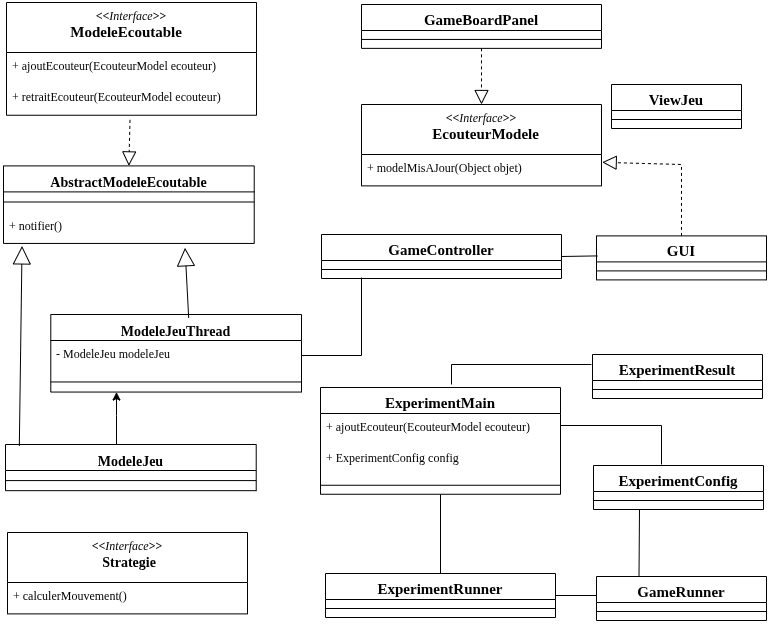
\includegraphics[width=1\linewidth, height=0.75\paperheight, keepaspectratio]{images/diagramme.png}
    \caption{Le diagramme UML des classes principales}
\end{figure}

\subsection{Architecture MVC}
L'application suit une logique proche du patron MVC. Le modèle correspond aux classes qui décrivent et font évoluer l'état du jeu, en particulier \texttt{ModeleJeu}, \texttt{Plateau}, \texttt{Player} et les classes de stratégie. La vue est constituée par les composants Swing, en particulier \texttt{GUI}, \texttt{GameBoardPanel}, \texttt{SidePanel}, \texttt{ControlSection} et \texttt{SpeedSection}. Le contrôleur principal, \texttt{GameController}, coordonne la création d'une partie, la relance d'une simulation, la lecture de l'historique et le déclenchement des actions utilisateur.

Ce découpage n'est pas purement théorique. Il se retrouve dans la manière dont le programme a été construit. Les règles du jeu et les calculs de stratégie ne dépendent pas directement des composants graphiques, ce qui permet de réutiliser le modèle dans les expérimentations sans passer systématiquement par l'interface. Cette séparation constitue un point fort du projet.


\subsection{Interactions entre les modules}

L'un des points forts de cette architecture est l'indépendance totale du \textbf{Modèle}. Celui-ci contient l'intégralité des règles et de la logique de simulation, lui permettant de fonctionner de manière autonome, sans nécessiter de contrôleur ou d'interface graphique.

\subsubsection{Flux en mode interactif (GUI)}
Lorsqu'une partie est lancée via l'interface utilisateur, le processus d'interaction suit une chaîne précise :
\begin{enumerate}
    \item \textbf{Configuration :} Le contrôleur récupère les paramètres (taille du plateau, types d'IA) depuis la boîte de configuration.
    \item \textbf{Initialisation :} Il instancie les objets \texttt{Player}, crée le \texttt{ModeleJeu} et lie ce dernier aux panneaux graphiques (\texttt{GameBoardPanel}, etc.).
    \item \textbf{Cycle de jeu :} À chaque tour, le modèle calcule ou reçoit les mouvements, met à jour l'état du \texttt{Plateau}, puis notifie automatiquement la vue via le pattern Observer pour déclencher le rafraîchissement visuel.
\end{enumerate}


\subsubsection{Flux en mode expérimental}
Dans le cadre du package \texttt{experiment}, l'enchaînement est analogue mais optimisé pour la performance brute. Le pilotage est assuré par les classes \texttt{ExperimentMain}, \texttt{ExperimentRunner} et \texttt{GameRunner}. 
\begin{itemize}
    \item \textbf{Exécution en série :} Ces classes instancient les joueurs et exécutent les parties en boucle sans aucune intervention de la \texttt{View}.
    \item \textbf{Collecte de données :} Les résultats de chaque simulation sont encapsulés dans des objets \texttt{GameResult} et agrégés dans un \texttt{ExperimentResult}.
    \item \textbf{Exploitation :} En fin de chaîne, les modules d'export et d'analyse transforment ces données brutes en fichiers CSV, rapports PDF ou graphiques statistiques.
\end{itemize}

Cette séparation permet d'utiliser le même moteur de règles pour deux usages radicalement différents : une démonstration visuelle fluide et une analyse statistique de masse.


\section{Modélisation du système}

\subsection{Pattern Observer}

Le patron Observer est utilisé pour relier le modèle à la vue. Les classes du package \texttt{observer}, telles que \texttt{ModeleEcoutable}, \texttt{AbstractModeleEcoutable} et \texttt{EcouteurModele}, permettent au modèle de notifier les composants intéressés lorsqu'une modification survient. Ainsi, lorsqu'un tour de jeu est exécuté et que le plateau change, la vue peut être rafraîchie automatiquement sans devoir interroger en permanence l'état du modèle.

Ce choix simplifie la synchronisation entre la logique de jeu et l'affichage. Il évite également de coupler trop fortement le modèle aux composants Swing, ce qui reste conforme à l'esprit d'une architecture modulaire.


\subsection{Package modele}

Le modèle du jeu repose sur une représentation discrète de l'espace. Le plateau est une grille composée de cellules identifiées par des positions. Chaque joueur occupe une position courante et appartient à une équipe. À chaque tour, il choisit une direction parmi les déplacements autorisés. Le déplacement a deux conséquences : la position du joueur change, et la case quittée devient une trace assimilée à un obstacle. Ce mécanisme suffit à créer la dynamique caractéristique de Tron, où l'espace se ferme progressivement.

Les décisions de déplacement dépendent de la stratégie associée au joueur. La stratégie peut se contenter d'un choix aléatoire, ou bien lancer une recherche de type MinMax, AlphaBeta, MaxN, Paranoid ou SOS. Dans tous les cas, l'évaluation intermédiaire des positions repose sur une heuristique. Le modèle combine donc deux niveaux : la stratégie décide comment explorer les coups possibles, tandis que l'heuristique donne une valeur aux positions intermédiaires.

\subsubsection{Classe Plateau}

La classe \texttt{Plateau} représente la surface de jeu. Elle stocke les dimensions de la grille, la structure des cellules et l'information nécessaire pour savoir si une case est libre, occupée ou interdite. Elle joue un rôle central, car toutes les stratégies utilisent le plateau pour connaître les coups possibles, simuler des mouvements ou évaluer l'espace encore libre. Dans le déroulement d'une partie, le plateau constitue donc la mémoire de l'environnement.

Son importance apparaît aussi dans les heuristiques. FreeSpace évalue les zones atteignables à partir du plateau courant, Voronoi s'appuie sur les distances aux cases libres pour répartir le territoire, et TreeOfChambers exploite la topologie de l'espace lorsqu'il se fragmente en régions. Le plateau ne sert donc pas seulement à l'affichage ; il soutient directement l'intelligence décisionnelle du système.

\subsubsection{Classe Cellule}

La classe \texttt{Cellule} permet de modéliser l'état élémentaire d'une case du plateau. Elle sert à distinguer les cases libres des cases déjà occupées ou transformées en obstacles. Associée à l'énumération \texttt{CellState}, elle fournit une représentation simple mais suffisante pour gérer l'évolution du jeu. Cette granularité est adaptée à Tron, où la notion de collision se réduit essentiellement à la question suivante : la case ciblée est-elle encore disponible au moment du déplacement.

\subsubsection{Classe Position}

La classe \texttt{Position} encapsule les coordonnées d'une case et fournit des opérations utiles, comme le calcul de distance de Manhattan ou la comparaison entre positions. Cette abstraction évite de manipuler partout de simples couples d'entiers. Elle améliore la lisibilité du code et facilite le traitement algorithmique, en particulier lorsque les stratégies génèrent des coups voisins, comparent des distances ou vérifient qu'une position appartient à la grille.

\subsubsection{Classe ModeleJeu}

\texttt{ModeleJeu} constitue la classe centrale du projet. Elle orchestre l'évolution d'une partie en maintenant le plateau, la liste des joueurs, l'état de vie de chacun, le déroulement des tours et les conditions d'arrêt. C'est elle qui applique réellement les déplacements et qui détermine si une collision entraîne l'élimination d'un joueur. Son rôle est également de servir de point d'appui à la vue et au contrôleur.

La classe concentre la logique métier du jeu. Elle ne se contente pas de stocker des données ; elle exprime la manière dont la partie progresse. C'est pourquoi la plupart des autres composants, qu'il s'agisse des stratégies, de l'interface ou des expérimentations, se structurent autour d'elle.

\section{Package Stratégie IA et ses composantes}

Le projet distingue clairement la stratégie de l'heuristique. Une stratégie définit la façon dont un joueur explore les coups possibles avant de prendre une décision. Une heuristique, quant à elle, sert à évaluer la qualité d'un état lorsque la profondeur maximale de recherche est atteinte ou lorsqu'il n'est pas pertinent d'explorer davantage. Cette séparation est incarnée dans le code par les interfaces et classes abstraites du package \texttt{model}, en particulier \texttt{Strategie}, \texttt{AbstractStrategie} et \texttt{Heuristic}.

Toutes les stratégies mises en place répondent au même objectif immédiat, à savoir choisir une direction de déplacement valable. En revanche, elles diffèrent par leur manière de représenter les adversaires et de raisonner sur l'avenir. Certaines suivent une logique classique de maximisation et de minimisation, alors que d'autres sont pensées pour le multi-joueur ou pour des comportements de coalition.

\subsection{Stratégie Minimax}

La stratégie Minimax cherche le coup qui donne la meilleure valeur au joueur courant en supposant qu'au niveau suivant le jeu évolue de la manière la plus défavorable. Dans le projet, la classe \texttt{MinMaxStrategie} copie le plateau, simule chaque déplacement possible, puis lance une recherche récursive jusqu'à une profondeur donnée. Quand la profondeur est atteinte, ou quand il n'y a plus de coup possible, l'état est évalué avec l'heuristique choisie.

Le fonctionnement peut être résumé par le pseudo-code suivant.

\begin{algorithm}[H]
\DontPrintSemicolon
\SetKwFunction{FMinimax}{minimax}
\SetKwFunction{FEval}{heuristic.evaluate}
\SetKwFunction{FGetCoups}{getCoupsPossibles}
\SetKwFunction{FCopy}{copierPlateau}
\SetKwFunction{FDeplacer}{deplacer}

\Fn{\FMinimax{plateau, player, depth, maximisant}}{
    
    \If{Temps écoulé \textbf{ou} depth == 0 \textbf{ou} \FGetCoups{pos} est vide}{
        \Return \FEval{plateau, player}\;
    }

    \If{maximisant}{
        bestValue $\leftarrow$ $-\infty$\;
        \For{chaque direction $dir$ \textbf{dans} \FGetCoups{pos}}{
            copiePlateau $\leftarrow$ \FCopy{plateau}\;
            \FDeplacer{copiePlayer, dir, copiePlateau}\;
            value $\leftarrow$ \FMinimax{copiePlateau, copiePlayer, depth - 1, faux}\;
            bestValue $\leftarrow$ max(bestValue, value)\;
        }
        \Return bestValue\;
    }
    \Else{
        worstValue $\leftarrow$ $+\infty$\;
        \For{chaque direction $dir$ \textbf{dans} \FGetCoups{pos}}{
            copiePlateau $\leftarrow$ \FCopy{plateau}\;
            \FDeplacer{copiePlayer, dir, copiePlateau}\;
            value $\leftarrow$ \FMinimax{copiePlateau, copiePlayer, depth - 1, vrai}\;
            worstValue $\leftarrow$ min(worstValue, value)\;
        }
        \Return worstValue\;
    }
}
\caption{Algorithme Minimax}
\end{algorithm}

\vspace{1cm}

Cette stratégie reste surtout adaptée aux situations proches du duel, car elle alterne simplement entre une phase où l'on maximise et une phase où l'on minimise.

\subsection{Stratégie Alpha-Beta}

La stratégie Alpha-Beta reprend l'idée de Minimax, mais elle coupe certaines branches de recherche dès qu'il devient clair qu'elles ne pourront pas améliorer le résultat final. Dans le code, la classe \texttt{AlphaBetaStrategie} commence par simuler chaque déplacement du joueur, cherche ensuite un adversaire vivant sur le plateau, puis lance une recherche récursive avec deux bornes, \texttt{alpha} et \texttt{beta}. Cette version est utilisée surtout dans le cas d'un affrontement simple.

Le pseudo-code correspondant est le suivant.

\begin{algorithm}[H]
\DontPrintSemicolon
\SetKwFunction{FAlphaBeta}{minimaxAlphaBeta}
\SetKwFunction{FEval}{heuristic.evaluate}

\Fn{\FAlphaBeta{plateau, me, opponent, depth, $\alpha$, $\beta$, maximizing}}{
    
    \If{temps écoulé \textbf{OR} depth $== 0$ \textbf{OR} terminal node}{
        \Return \FEval{plateau, me}\;
    }

    \If{maximizing}{
        $value \leftarrow -\infty$\;
        \For{chaque direction $dir$ \textbf{in} coups}{
            simulation $\leftarrow$ copier(plateau)\;
            simulerMouvement(simulation, me, dir)\;
            
            eval $\leftarrow$ \FAlphaBeta{simulation, me, opponent, depth - 1, $\alpha$, $\beta$, false}\;
            
            $value \leftarrow \max(value, eval)$\;
            $\alpha \leftarrow \max(\alpha, value)$\;
            
            \If{$\beta \le \alpha$}{
                \textbf{break} \tcp*{Élagage Alpha}
            }
        }
        \Return $value$\;
    }
    \Else{
        $value \leftarrow +\infty$\;
        \For{chaque direction $dir$ \textbf{in} coups}{
            simulation $\leftarrow$ copier(plateau)\;
            simulerMouvement(simulation, opponent, dir)\;
            
            eval $\leftarrow$ \FAlphaBeta{simulation, me, opponent, depth - 1, $\alpha$, $\beta$, true}\;
            
            $value \leftarrow \min(value, eval)$\;
            $\beta \leftarrow \min(\beta, value)$\;
            
            \If{$\beta \le \alpha$}{
                \textbf{break} \tcp*{Élagage Beta}
            }
        }
        \Return $value$\;
    }
}
\caption{Minimax avec élagage Alpha-Beta}
\end{algorithm}
\vspace{1cm}

L'avantage principal de cette stratégie est de garder une logique proche de Minimax tout en évitant une partie des calculs inutiles.


\subsection{Stratégie Paranoid}

La stratégie Paranoid suppose que tous les autres joueurs cherchent ensemble à faire perdre le joueur courant. Dans le projet, la classe \texttt{ParanoidStrategie} récupère d'abord la liste des joueurs encore vivants. Elle teste ensuite chaque coup du joueur principal, puis alterne entre une étape où ce joueur cherche à maximiser sa valeur et une étape où l'ensemble des autres joueurs cherche à la minimiser. Le principe reste proche d'Alpha-Beta, mais la partie minimisante parcourt tous les adversaires.

Le pseudo-code peut être écrit ainsi.


\begin{algorithm}[H]
\DontPrintSemicolon
\SetKwFunction{FParanoid}{paranoid}
\SetKwFunction{FEval}{heuristic.evaluate}

\Fn{\FParanoid{plateau, me, depth, $\alpha$, $\beta$, maximiserJoueur}}{

    \If{depth $== 0$ \textbf{OR} \textbf{NOT} me.isAlive()}{
        \Return \FEval{plateau, me}\;
    }

    \If{maximiserJoueur}{
        $maxVal \leftarrow -\infty$\;
        coups $\leftarrow$ plateau.getCoupsPossibles(me.pos)\;
        \If{coups est vide}{
            \Return \FEval{plateau, me}\;
        }
        \For{chaque direction $dir$ \textbf{dans} coups}{
            plateauCopie $\leftarrow$ simulerCoup(plateau, me, dir)\;
            $val \leftarrow$ \FParanoid{plateauCopie, me, depth - 1, $\alpha$, $\beta$, \textbf{false}}\;
            $maxVal \leftarrow \max(maxVal, val)$\;
            $\alpha \leftarrow \max(\alpha, maxVal)$\;
            \If{$\beta \le \alpha$}{
                \textbf{break}\;
            }
        }
        \Return $maxVal$\;
    }
    \Else{
        $minVal \leftarrow +\infty$\;
        \ForEach{joueur $p$ \textbf{dans} joueurs}{
            \If{$p == me$ \textbf{OR} \textbf{NOT} $p$.isAlive()}{
                \textbf{continue}\;
            }
            \For{chaque direction $dir$ \textbf{dans} p.getCoupsPossibles()}{
                plateauCopie $\leftarrow$ simulerCoup(plateau, $p$, dir)\;
                $val \leftarrow$ \FParanoid{plateauCopie, me, depth - 1, $\alpha$, $\beta$, \textbf{true}}\;
                $minVal \leftarrow \min(minVal, val)$\;
                $\beta \leftarrow \min(\beta, minVal)$\;
                \If{$\beta \le \alpha$}{
                    \textbf{break} \tcp*{Élagage paranoïaque}
                }
            }
        }
        \Return $minVal$\;
    }
}
\caption{Algorithme Paranoid avec élagage Alpha-Beta}
\end{algorithm}

Cette manière de faire est simple à interpréter : le joueur agit comme s'il était seul contre tous.

\subsection{Stratégie SOS}

La stratégie SOS est pensée pour les situations multi-joueurs où l'on veut conserver une évaluation pour chaque joueur au lieu de ramener tout le monde à un simple duel. Dans le projet, la classe \texttt{SOSStrategie} teste les coups possibles du joueur de départ, puis lance une recherche récursive qui retourne un vecteur de scores. À chaque niveau, le joueur courant choisit la branche qui améliore le plus sa propre composante dans ce vecteur.

Le pseudo-code simplifié est le suivant.

C'est une variante intéressante ! Ton algorithme SOS (ou Socially Optimal Strategy / Simple Opponent Search) pour les jeux multi-joueurs ne retourne plus une valeur unique, mais un vecteur d'utilité (un score par joueur). Ici, le joueur courant cherche à maximiser sa propre composante dans ce vecteur. \\



\begin{algorithm}[H]
\DontPrintSemicolon
\SetKwFunction{FSOS}{sos}
\SetKwFunction{FUtil}{utiliteSociale}
\SetKwFunction{FEval}{heuristic.evaluate}
\SetKwFunction{FNext}{nextPlayer}

\Fn{\FSOS{plateau, depth, player}}{

    \If{depth $== 0$ \textbf{OR} coupsPossibles est vide}{
        evaluation $\leftarrow$ \FEval{plateau, player}\;
        \Return \FUtil{evaluation}\;
    }

    id $\leftarrow$ joueurs.indexOf(player)\;
    bestScore $\leftarrow$ $-\infty$\;
    bestVecteur $\leftarrow$ \FUtil{$-\infty$}\;

    \For{chaque direction $dir$ \textbf{dans} plateau.getCoupsPossibles()}{
        plateauCopie $\leftarrow$ copier(plateau)\;
        simulerMouvement(plateauCopie, player, dir)\;
        
        currentVecteur $\leftarrow$ \FSOS{plateauCopie, depth - 1, \FNext{playerCopie}}\;

        \If{currentVecteur[id] $>$ bestScore}{
            bestScore $\leftarrow$ currentVecteur[id]\;
            bestVecteur $\leftarrow$ currentVecteur\;
        }
    }

    \Return bestVecteur\;
}
\caption{Algorithme SOS (Socially Optimal Strategy)}
\end{algorithm}


Dans cette version, la fonction d'utilité sociale recopie la même valeur pour tous les joueurs. L'intérêt de cette stratégie est surtout de poser une base pour raisonner autrement qu'avec un simple max contre min.

\subsection{Élagage dans MAXN}

La stratégie MaxN est utilisée quand plusieurs joueurs prennent part au jeu et que chacun cherche à améliorer sa propre valeur. Dans le projet, la classe \texttt{MaxNStrategie} utilise un parallélisme à la racine : chaque coup possible du joueur de départ est évalué dans une tâche séparée, puis l'algorithme récursif \texttt{maxN} retourne un vecteur contenant une valeur pour chaque joueur. Le joueur courant choisit toujours la branche qui maximise sa propre case dans ce vecteur.

Le pseudo-code simplifié de cette stratégie est le suivant.

\begin{algorithm}[H]
\DontPrintSemicolon
\SetKwFunction{FMaxN}{maxN}
\SetKwFunction{FEvalAll}{evaluateAll}
\SetKwFunction{FShuffle}{shuffle}

\Fn{\FMaxN{plateau, players, depth, currentIndex}}{

    \If{depth $== 0$ \textbf{OR} timeExceeded()}{
        \Return \FEvalAll{plateau, players}\;
    }

    current $\leftarrow$ players.get(currentIndex)\;
    
    \If{\textbf{NOT} current.isAlive()}{
        \Return \FMaxN{plateau, players, depth, (currentIndex + 1) \% players.size()}\;
    }

    coups $\leftarrow$ plateau.getCoupsPossibles(current.pos)\;
    \FShuffle{coups}\;

    \If{coups est vide}{
        \Return \FEvalAll{plateau, players}\;
    }

    bestVector $\leftarrow$ \textbf{null}\;
    bestValue $\leftarrow$ $-\infty$\;

    \For{chaque direction $dir$ \textbf{dans} coups}{
        grid $\leftarrow$ copier(plateau)\;
        simulerMouvement(grid, current, dir)\;
        
        nextIndex $\leftarrow$ (currentIndex + 1) \% players.size()\;
        values $\leftarrow$ \FMaxN{grid, nextPlayers, depth - 1, nextIndex}\;

        \If{values[currentIndex] $>$ bestValue}{
            bestValue $\leftarrow$ values[currentIndex]\;
            bestVector $\leftarrow$ values\;
        }
    }

    \Return bestVector\;
}
\caption{Algorithme MaxN pour $n$ joueurs}
\end{algorithm}

Dans cette stratégie, il n'y a pas un élagage Alpha-Beta classique. En revanche, le projet essaie quand même de réduire le coût en limitant le parallélisme au premier niveau de l'arbre.

\section{Heuristiques}

\subsection{Principe des heuristiques}

Dans un jeu comme Tron, il est impossible d'explorer tous les coups possibles dès que le plateau ou le nombre de joueurs devient plus grand. Les heuristiques jouent donc un rôle central. Elles permettent d'estimer la qualité d'une position intermédiaire en attribuant une note à l'état du plateau. Cette note sert ensuite de base aux stratégies pour comparer les coups possibles lorsqu'elles atteignent leur profondeur limite.

Le projet implémente trois heuristiques distinctes. Leur coexistence permet d'étudier non seulement la qualité intrinsèque d'une stratégie de recherche, mais aussi la façon dont elle dépend d'une bonne évaluation locale des états.

\subsection{FreeSpace Heuristic}

L'heuristique FreeSpace mesure simplement combien de cases libres restent accessibles à partir de la position du joueur. Dans le projet, cette estimation est obtenue avec un parcours en largeur à partir de la case courante. Si le joueur est déjà éliminé, une très mauvaise valeur est renvoyée immédiatement. Cette heuristique est simple, rapide et facile à comprendre.

Le pseudo-code correspondant est le suivant.

\begin{algorithm}[H]
\DontPrintSemicolon
\SetKwFunction{FEval}{evaluate}
\SetKwFunction{FCount}{countAccessibleCells}
\SetKwData{Grid}{plateau}
\SetKwData{Pos}{pos}

\SetKwBlock{Begin}{Début}{}

\Fn{\FEval{\Grid, joueur}}{
    \If{\textbf{NOT} joueur.isAlive()}{
        \Return $-1000000$\;
    }
    \Return \FCount{\Grid, joueur.pos}\;
}

\BlankLine

\Fn{\FCount{\Grid, positionInitiale}}{
    \If{\textbf{NOT} \Grid.estDansPlateau(positionInitiale)}{
        \Return 0\;
    }
    
    $compteur \leftarrow 0$\;
    $visite \leftarrow$ Matrice booléenne $[L][C]$ initialisée à \textbf{false}\;
    $file \leftarrow$ File vide\;
    
    $file.enfiler(positionInitiale)$\;
    $visite[positionInitiale.lig][positionInitiale.col] \leftarrow \textbf{true}$\;
    
    \While{$file$ n'est pas vide}{
        $courant \leftarrow file.defiler()$\;
        $compteur \leftarrow compteur + 1$\;
        
        \ForEach{direction $dir$ \textbf{dans} \{HAUT, BAS, GAUCHE, DROITE , NONE\}}{
            $voisin \leftarrow courant.deplacer(dir)$\;
            
            \If{\Grid.estDansPlateau($voisin$) \textbf{AND} \textbf{NOT} $visite[voisin.lig][voisin.col]$}{
                \If{\Grid.estLibre($voisin$)}{
                    $visite[voisin.lig][voisin.col] \leftarrow \textbf{true}$\;
                    $file.enfiler($voisin$)$\;
                }
            }
        }
    }
    \Return $compteur$\;
}
\caption{Heuristique d'Espace Libre (BFS)}
\end{algorithm}

Cette méthode donne une bonne première approximation, mais elle ne distingue pas vraiment un espace sécurisé d'un espace qui sera bientôt perdu.

\subsection{Voronoi Heuristic}

L'heuristique Voronoi cherche à estimer le territoire que chaque joueur pourra contrôler. Pour cela, elle lance une propagation simultanée à partir de la position de tous les joueurs vivants. Chaque case libre est attribuée à l'équipe du joueur qui l'atteint le plus vite. Si deux équipes arrivent exactement en même temps, la case est marquée comme contestée et n'est attribuée à personne. Le score final correspond à la différence entre le territoire de l'équipe du joueur et celui des autres équipes.

Le pseudo-code simplifié est le suivant.

\begin{algorithm}[H]
\DontPrintSemicolon
\SetKwFunction{FEval}{evaluate}
\SetKwData{Grid}{plateau}
\SetKwData{Dist}{distance}
\SetKwData{Owner}{proprietaireEquipe}
\SetKwData{Inf}{$\infty$}

\Fn{\FEval{\Grid, joueur}}{
    \If{\textbf{NOT} joueur.isAlive()}{
        \Return $-1000000$\;
    }

    $L \leftarrow$ \Grid.nbLignes \tcp*{Initialisation des structures}
    $C \leftarrow$ \Grid.nbColonnes\;
    \Dist $\leftarrow$ Tableau de taille $L \times C$ rempli de \Inf\;
    \Owner $\leftarrow$ Tableau de taille $L \times C$ rempli de \texttt{null}\;
    $file \leftarrow$ File vide\;

    \tcp{Identification des sources (têtes des joueurs)}
    \ForEach{case $p$ du \Grid}{
        $occupant \leftarrow$ \Grid.getJoueurAt($p$)\;
        \If{$occupant \neq \texttt{null}$}{
            \Dist[$p$] $\leftarrow 0$\;
            \Owner[$p$] $\leftarrow occupant.team$\;
            $file.enfiler(p)$\;
        }
    }

    \tcp{Propagation multi-source (BFS)}
    \While{$file$ n'est pas vide}{
        $courant \leftarrow file.defiler()$\;
        $equipeCourante \leftarrow$ \Owner[$courant$]\;
        
        \If{$equipeCourante == \texttt{null}$}{ \textbf{continue}\; } \tcp{Case contestée}

        \ForEach{direction $dir$}{
            $voisin \leftarrow courant.deplacer(dir)$\;
            \If{\Grid.estDansPlateau($voisin$) \textbf{AND} \Grid.estLibre($voisin$)}{
                \If{\Dist[$voisin$] $== \Inf$}{
                    \Dist[$voisin$] $\leftarrow$ \Dist[$courant$] $+ 1$\;
                    \Owner[$voisin$] $\leftarrow$ $equipeCourante$\;
                    $file.enfiler(voisin)$\;
                }
                \ElseIf{\Dist[$voisin$] $==$ \Dist[$courant$] $+ 1$ \textbf{AND} \Owner[$voisin$] $\neq$ $equipeCourante$}{
                    \Owner[$voisin$] $\leftarrow \texttt{null}$ \tcp*{Égalité : case contestée}
                }
            }
        }
    }

    \tcp{Calcul du score final}
    $scoreEquipe \leftarrow 0$, $scoreAdversaires \leftarrow 0$\;
    \ForEach{case $c$ dans \Owner}{
        \If{$c == joueur.team$}{ $scoreEquipe \leftarrow scoreEquipe + 1$\; }
        \ElseIf{$c \neq \texttt{null}$}{ $scoreAdversaires \leftarrow scoreAdversaires + 1$\; }
    }

    \Return $(scoreEquipe - scoreAdversaires)$\;
}
\caption{Heuristique de Voronoi (Partition du Territoire)}
\end{algorithm}

Cette heuristique est plus riche que FreeSpace, car elle tient compte de la concurrence entre joueurs pour l'occupation de l'espace.

\subsection{Tree Of Chambers Heuristic}

L'heuristique Tree Of Chambers essaie de mieux comprendre la structure du plateau quand l'espace commence à se couper en zones séparées. Dans le projet, cette heuristique suit plusieurs étapes. Elle commence par repérer l'adversaire le plus proche, construit ensuite une partition de type Voronoi à deux joueurs, puis cherche les points d'articulation, c'est-à-dire les cases qui relient plusieurs régions. À partir de là, elle estime la taille de la chambre principale et la meilleure chambre voisine accessible.

Le pseudo-code simplifié ci-dessous reprend cette logique générale.

\begin{algorithm}[H]
\DontPrintSemicolon
\SetKwFunction{FEval}{evaluate}
\SetKwFunction{FToC}{tocValue}
\SetKwFunction{FArtic}{findArticulationPoints}
\SetKwFunction{FExplore}{exploreChamber}

\Fn{\FEval{plateau, joueur}}{
    \If{\textbf{NOT} joueur.isAlive()}{ \Return $-10^{6}$\; }
    
    $adversaires \leftarrow$ plateau.getOpponents(joueur)\;
    $monScore \leftarrow 0, scoreAdverse \leftarrow 0$\;
    
    \ForEach{adversaire $opp$}{
        $V \leftarrow$ calculerVoronoi2P(plateau, joueur, $opp$)\;
        $monScore \leftarrow \max(monScore, \FToC(V, \text{joueur}))$\;
        $scoreAdverse \leftarrow \max(scoreAdverse, \FToC(V, \text{opp}))$\;
    }
    \Return $monScore - scoreAdverse$\;
}

\BlankLine

\Fn{\FToC{voronoi, p}}{
    $region \leftarrow$ voronoi.getRegion(p)\;
    $articul \leftarrow$ \FArtic{$region$}\;
    
    \tcp{Chambre principale (contenant la tête du joueur)}
    $main \leftarrow$ \FExplore($region, articul, p.pos$)\;
    
    $bestAdj \leftarrow 0$\;
    \ForEach{point $a \in main.pointsArticulation$}{
        $ch \leftarrow$ \FExplore($region, articul, a$)\;
        \If{\textbf{NOT} $ch.touchesBattlefront$}{
            $bestAdj \leftarrow \max(bestAdj, ch.size)$\;
        }
    }
    \Return $main.size + bestAdj$\;
}
\caption{Heuristique Tree of Chambers (ToC)}
\end{algorithm}

Cette heuristique est plus coûteuse, mais elle essaie de mieux représenter les situations où le plateau est découpé en couloirs et en zones presque fermées.


\section{Package view}

Le package \texttt{view} regroupe l’ensemble des composants graphiques du projet. L’interface a été développée en \textbf{Swing} autour d’une fenêtre principale et de plusieurs panneaux spécialisés. L’objectif n’était pas seulement de proposer un affichage du jeu, mais aussi de fournir un véritable espace de configuration et d’observation. La classe \texttt{GUI} centralise l’assemblage de ces composants. L’interface permet ainsi de lancer une partie, d’en suivre l’évolution visuellement et d’agir sur certains paramètres d’exécution comme la vitesse ou la pause.

Cette interface joue un rôle important dans la compréhension du projet, car elle rend immédiatement visibles les effets des stratégies mises en place. Elle transforme donc le simulateur en outil pédagogique, mais aussi en support d’expérimentation.

\subsection{Architecture de l'interface d'affichage des expérimentations}

L’interface graphique a été développée en utilisant \textbf{Swing} et \textbf{JFreeChart} afin d’offrir une visualisation claire et interactive des résultats des expérimentations. Elle est organisée autour d’une fenêtre principale et de plusieurs panneaux spécialisés. Cette structure permet de séparer les zones d’affichage, de configuration et de contrôle.

La classe \texttt{GameBoardPanel} est le composant chargé de représenter graphiquement le plateau et les déplacements des joueurs. Elle affiche les cellules, les traces laissées sur la grille ainsi que les positions courantes des agents. Son fonctionnement repose sur les notifications envoyées par le modèle, ce qui permet de mettre à jour l’affichage au fur et à mesure que la partie progresse. Ce panneau rend la dynamique du jeu plus lisible et permet de comprendre rapidement si une stratégie adopte un comportement d’évitement, d’occupation du territoire ou de confrontation directe.

La classe \texttt{SidePanel} regroupe les éléments annexes à l’affichage principal. Elle sert de conteneur aux différentes sections de contrôle et d’information. Cette organisation améliore l’ergonomie générale de la fenêtre en séparant clairement la zone de jeu de la zone de commande. Ce choix de structuration se retrouve dans l’ensemble du package \texttt{view} et permet d’ajouter ou de modifier une partie de l’interface sans devoir réécrire entièrement la fenêtre principale.

La classe \texttt{ControlSection} rassemble les commandes de pilotage de la partie, en particulier le lancement, la pause et la relance. Ce composant joue un rôle pratique essentiel, car il relie directement l’utilisateur au contrôleur. Il participe à la dimension interactive du projet et facilite les tests manuels des stratégies.

La classe \texttt{SpeedSection} permet d’ajuster la vitesse d’exécution de la simulation. Cette fonctionnalité est particulièrement utile pour observer le comportement des algorithmes. Une vitesse élevée convient aux tests rapides, tandis qu’une exécution plus lente rend possible une analyse visuelle plus fine des déplacements et des décisions successives.

\subsection{Architecture de l'interface des expérimentations}

En complément de l’interface du jeu, une interface dédiée aux expérimentations a également été développée. Elle avait pour objectif de faciliter le lancement des campagnes de tests et l’observation des résultats obtenus. La fenêtre principale sert de conteneur pour tous les panneaux et composants de cette interface. Elle offre une vue d’ensemble des résultats des expérimentations et permet de naviguer entre les différentes sections de configuration et de visualisation.

\begin{center}
    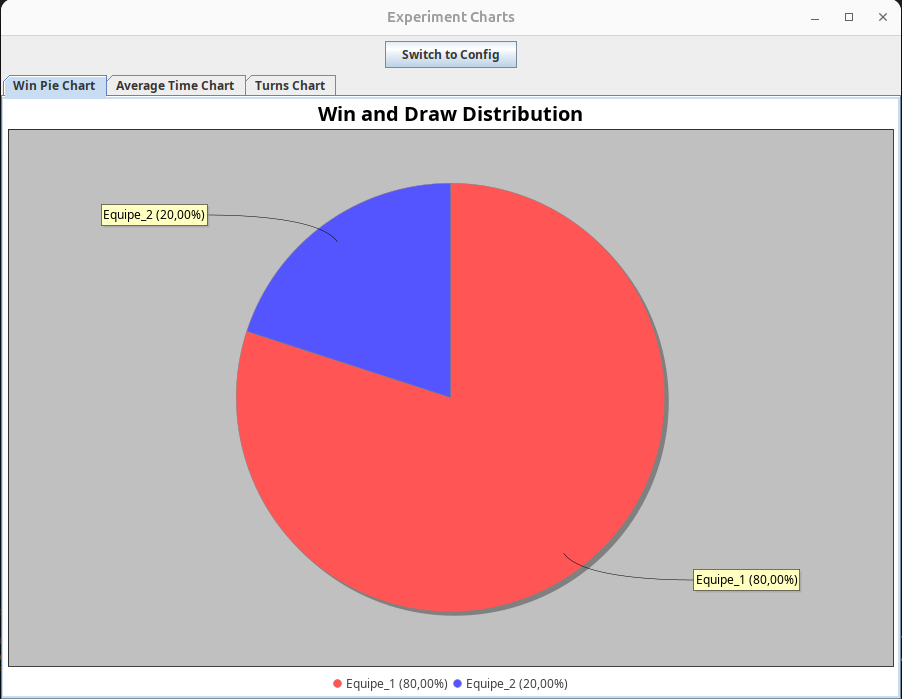
\includegraphics[width=0.6\textwidth]{images/Capture d’écran du 2026-03-26 16-53-57.png}
    
    \text{Exemple de fenêtre principale de l’interface}
\end{center}

Une partie importante de cette interface est consacrée à la configuration. Elle permet de définir les paramètres des expérimentations, comme la taille du plateau, le nombre d’équipes, les stratégies, les heuristiques et le nombre de parties à exécuter. Cette partie donne donc une certaine souplesse pour préparer plusieurs campagnes de tests sans devoir modifier directement le code.

\begin{center}
    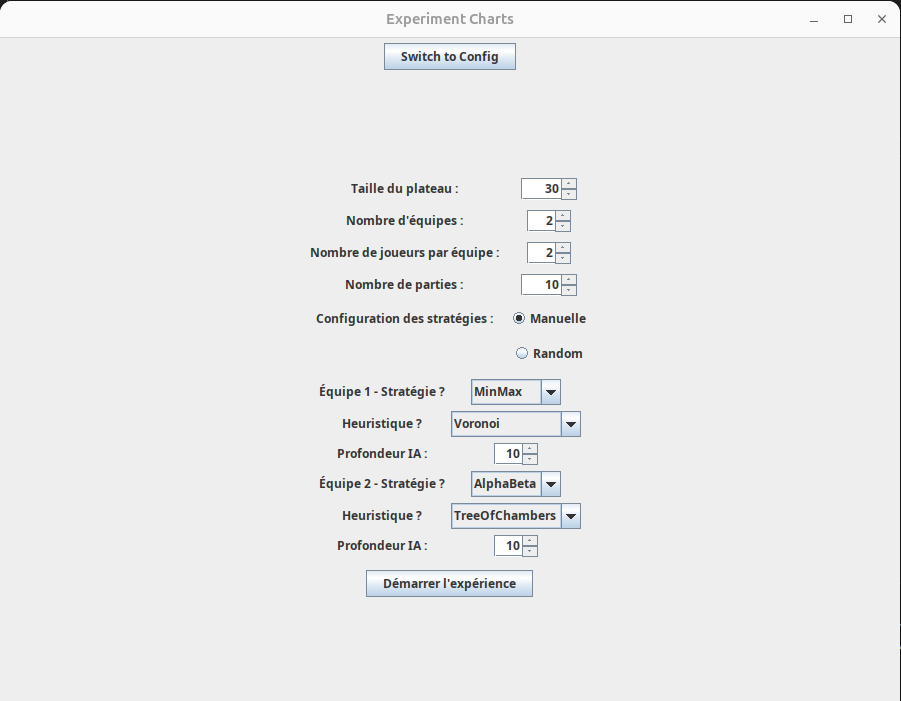
\includegraphics[width=0.6\textwidth]{images/Capture d’écran du 2026-03-26 16-52-18.png}
    
    \text{Exemple de panneau de configuration}
\end{center}

L’interface comporte également une partie dédiée à la visualisation. Celle-ci s’appuie sur \textbf{JFreeChart} pour afficher les résultats sous forme de graphiques, par exemple des diagrammes circulaires ou des histogrammes. Ce choix rend la lecture des statistiques plus simple et permet de comparer plus rapidement les configurations testées.

\vspace{-10}
\begin{figure}[h]
    \centering
    \begin{subfigure}{0.45\textwidth}
        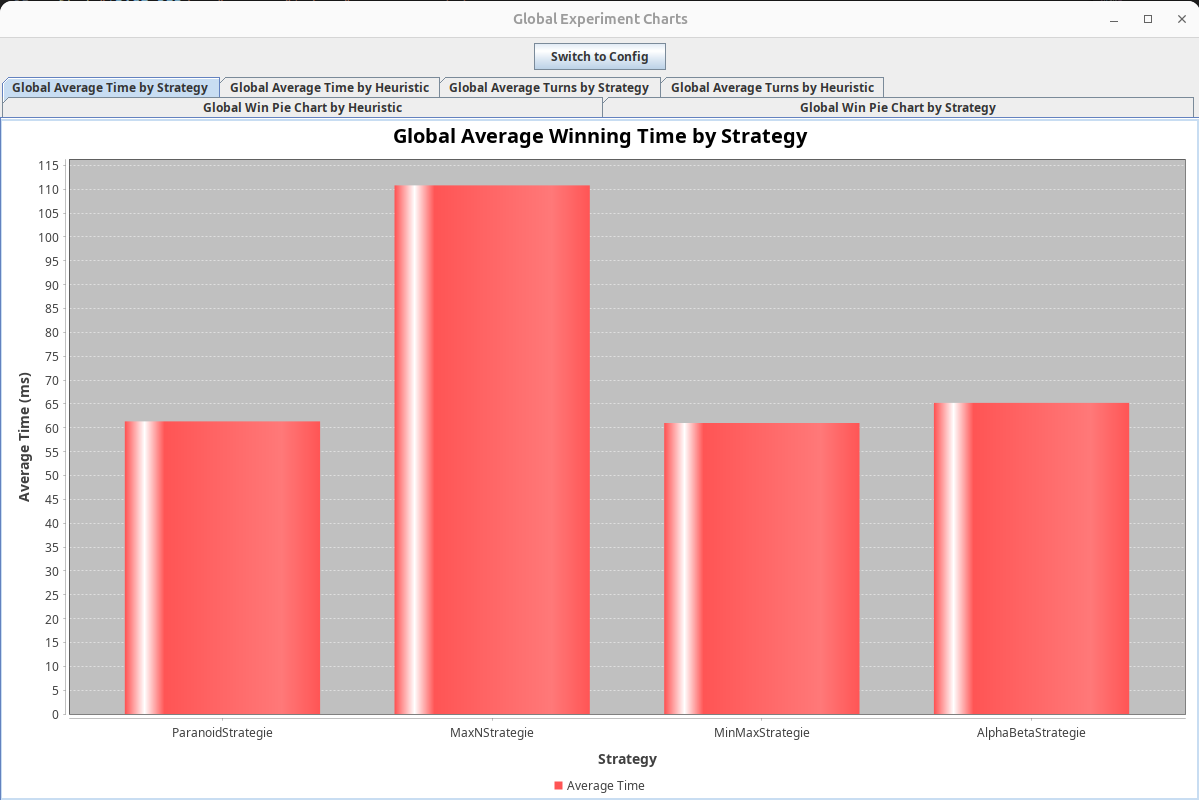
\includegraphics[width=\linewidth]{images/Capture d’écran du 2026-03-26 13-23-08.png}
        \caption{Exemple de graphique statistique}
    \end{subfigure}
    \hfill
    \begin{subfigure}{0.45\textwidth}
        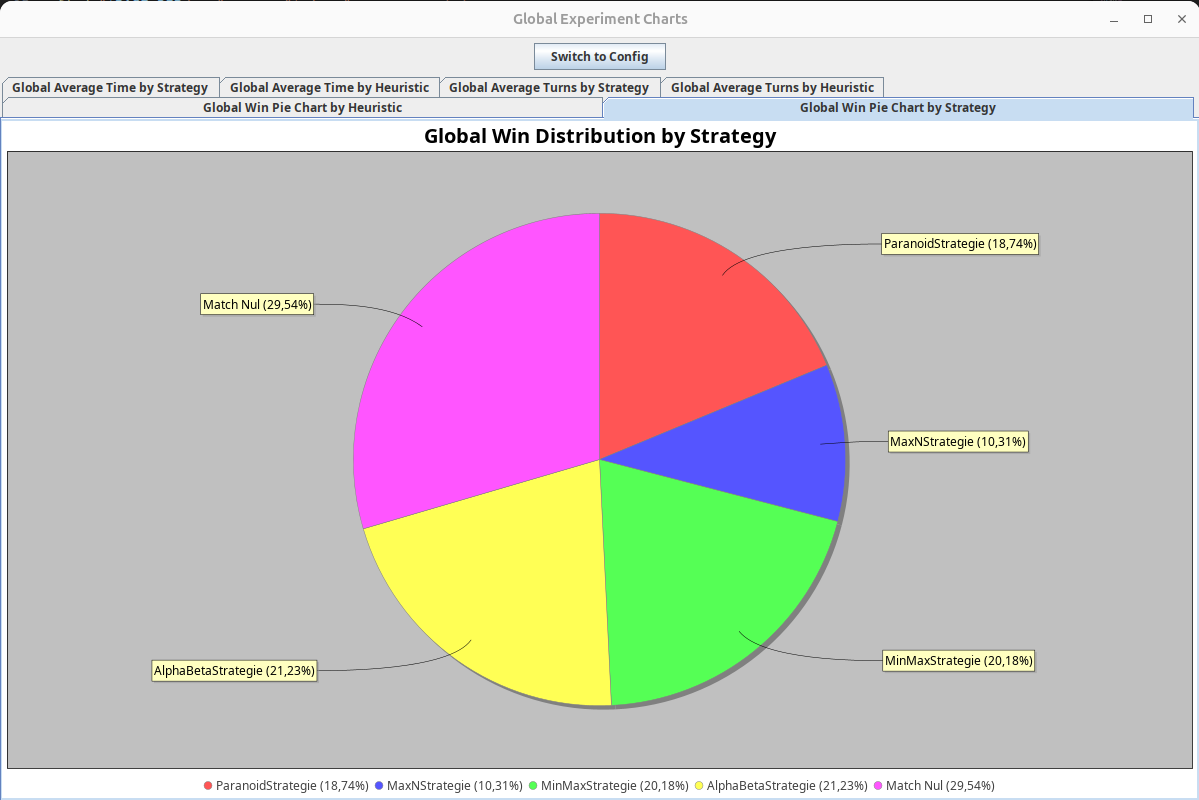
\includegraphics[width=\linewidth]{images/Capture d’écran du 2026-03-26 13-24-48.png}
        \caption{Visualisation des résultats par configuration}
    \end{subfigure}

    \vspace{5mm}

    \begin{subfigure}{0.45\textwidth}
        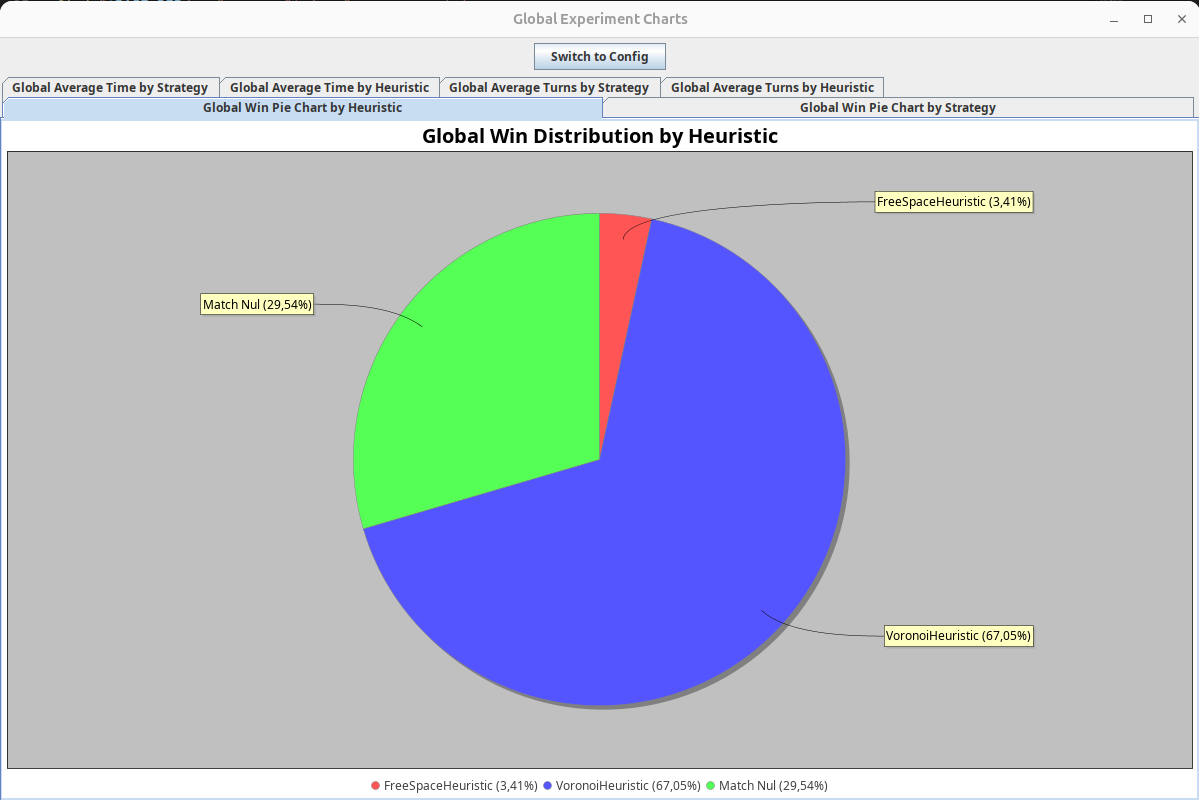
\includegraphics[width=\linewidth]{images/Capture d’écran du 2026-03-26 13-24-35.png}
        \caption{Exemple de comparaison graphique}
    \end{subfigure}
    \hfill
    \begin{subfigure}{0.45\textwidth}
        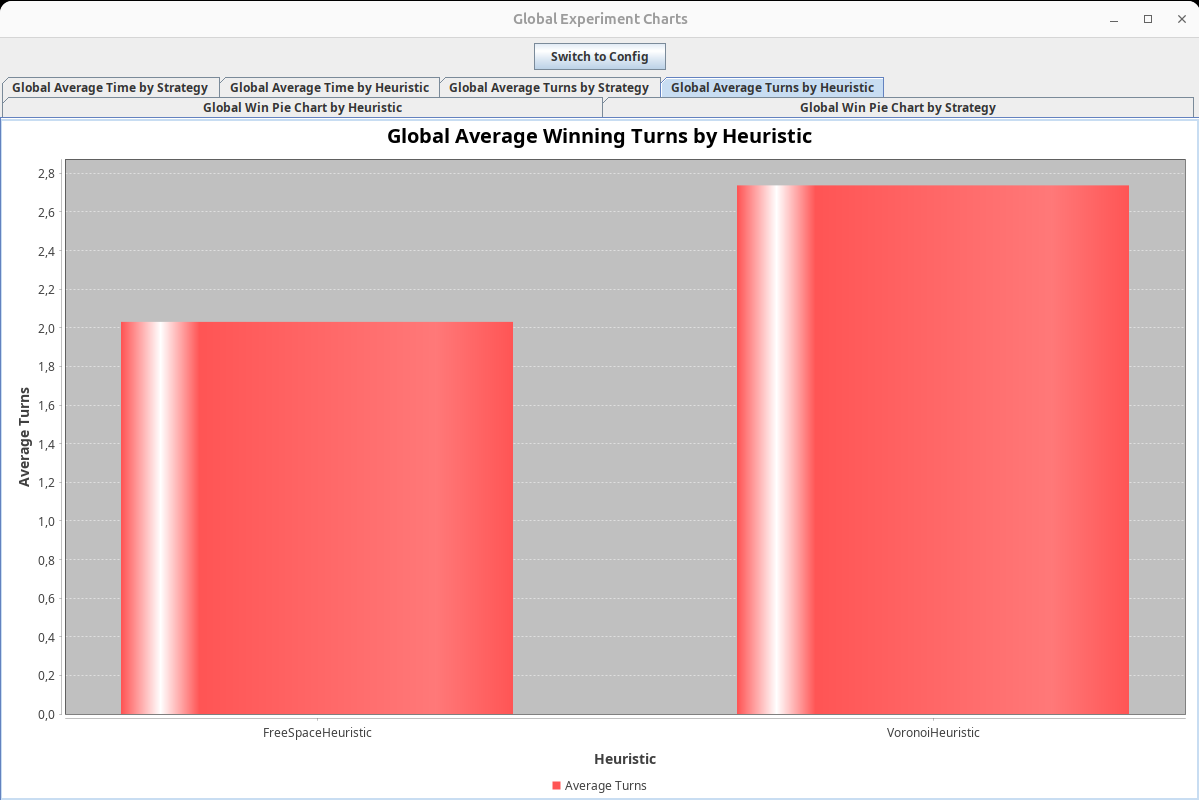
\includegraphics[width=\linewidth]{images/Capture d’écran du 2026-03-26 13-25-41.png}
        \caption{Autre exemple d’affichage des résultats}
    \end{subfigure}
    \caption{Exemples d’écrans de l’interface d’analyse des expérimentations}
    \label{fig:interface_experimentations}
\end{figure}

\subsubsection{Fonctionnalités}

L’outil d’analyse permettait d’abord de lancer les expérimentations automatiquement à partir des paramètres choisis. Une fois la configuration définie, les parties étaient exécutées en arrière-plan, ce qui évitait de devoir les lancer une par une manuellement. Cela rendait possible l’exécution d’un grand nombre de tests dans un temps raisonnable.

Il permettait ensuite d’afficher les résultats obtenus de manière lisible. Les données produites après les expériences étaient regroupées sous forme de statistiques et de graphiques. Cela aidait à comparer plus facilement les stratégies, les heuristiques, les profondeurs de recherche ou encore les tailles de plateau.

Enfin, l’outil facilitait aussi la gestion des configurations. Il était possible de modifier les paramètres des expériences, de relancer de nouvelles campagnes de tests et d’essayer différentes combinaisons de stratégies et d’heuristiques. Cette souplesse permettait d’explorer plusieurs scénarios sans avoir à changer manuellement tout le code à chaque fois.

\subsubsection{Évolution}

Cette interface d’affichage a constitué notre première approche pour la visualisation des données et des statistiques. Cependant, nous avons rencontré certaines limites en termes de performance et de capacité de traitement, notamment à cause de la complexité des données et du temps de calcul nécessaire pour les expérimentations à grande échelle.

Ces difficultés nous ont conduits à explorer une solution complémentaire en utilisant un code \textbf{Python} pour le traitement des données et la génération de graphiques. Cette approche s’est révélée plus adaptée pour analyser un grand volume de résultats. Nous avons néanmoins conservé cette partie dans le projet : même si elle ne correspond pas à l’outil principal retenu pour l’analyse finale, elle reste fonctionnelle et fait partie du travail réalisé.


\section{Exploitation et Expérimentations}

Cette section détaille les différentes manières d'interagir avec le logiciel, depuis l'utilisation interactive jusqu'à l'analyse automatisée de données de masse.

\subsection{Méthodes de lancement et Automatisation}
Le projet s'appuie sur l'outil d'automatisation \textbf{Apache Ant} pour gérer le cycle de vie de l'application. Un fichier de configuration \texttt{build.xml} définit plusieurs cibles (\textit{targets}) permettant de compiler, tester et lancer le projet de manière standardisée.

Le projet dispose d'un système d'automatisation à deux niveaux : \textbf{Ant} pour la gestion du cycle de vie logiciel (compilation, JAR, tests) et un \textbf{Script Shell} pour le pilotage intensif des campagnes d'expérimentation.

L'outil Ant permet non seulement de compiler, mais aussi de personnaliser les lancements via des arguments système. Les cibles principales sont :


\begin{description}
    \item[\texttt{ant compile} :] Prépare l'arborescence de construction (\texttt{build/}) et compile l'intégralité des sources Java ainsi que les classes de test en respectant.
    
    \item[\texttt{ant test} :] Exécute de manière automatisée la suite de tests unitaires JUnit. Les résultats sont exportés dans un dossier de rapport dédié.
    
    \item[\texttt{ant dist} :] Génère une archive exécutable \texttt{.jar} dans le dossier \texttt{dist/}. Cette cible inclut également la génération de la \textbf{Javadoc} pour documenter le projet.
    
    \item[\texttt{ant run} :] La cible par défaut. Elle compile le projet, génère le JAR et lance l'exécution principale.
    
    \item[\texttt{ant clean} :] Nettoie le répertoire de travail en supprimant les fichiers compilés, les distributions et la documentation générée.
\end{description}

\subsubsection{Script Shell d'Expérimentation Massive}

Pour évaluer l'efficacité des algorithmes, un script Shell (\texttt{script.sh}) a été développé. Il permet d'automatiser des milliers de duels en faisant varier systématiquement tous les paramètres du moteur de jeu.

\begin{itemize}
    \item \textbf{Exploration combinatoire :} Le script itère sur plusieurs tailles de plateaux ($10 \times 10$ à $20 \times 20$), plusieurs profondeurs de recherche (3, 6, 9) et croise toutes les stratégies (\textit{Minimax, AlphaBeta, MaxN, Paranoid et SOS}) avec toutes les heuristiques (\textit{Voronoi, Tree of Chambers, etc.}).
    \item \textbf{Gestion des données :} Pour chaque configuration, 50 parties sont jouées. Le script agrège les résultats dans un fichier \textbf{CSV} et fusionne les rapports PDF individuels.
  
\end{itemize}

\begin{quote}
    \textit{Avantage notable :} Cette automatisation permet de transformer des données brutes en une étude comparative rigoureuse sans intervention humaine, facilitant ainsi l'identification des configurations d'IA les plus performantes.
\end{quote}


\subsection{Interface console}
L'interface en ligne de commande sert de base technique au projet. Elle permet de suivre le déroulement d'une partie via des logs textuels détaillés. En mode console, ce qui facilite le débuggage rapide de la logique de mouvement et des scores sans la charge processeur liée au rendu graphique.

\begin{figure}[H]
    \centering
    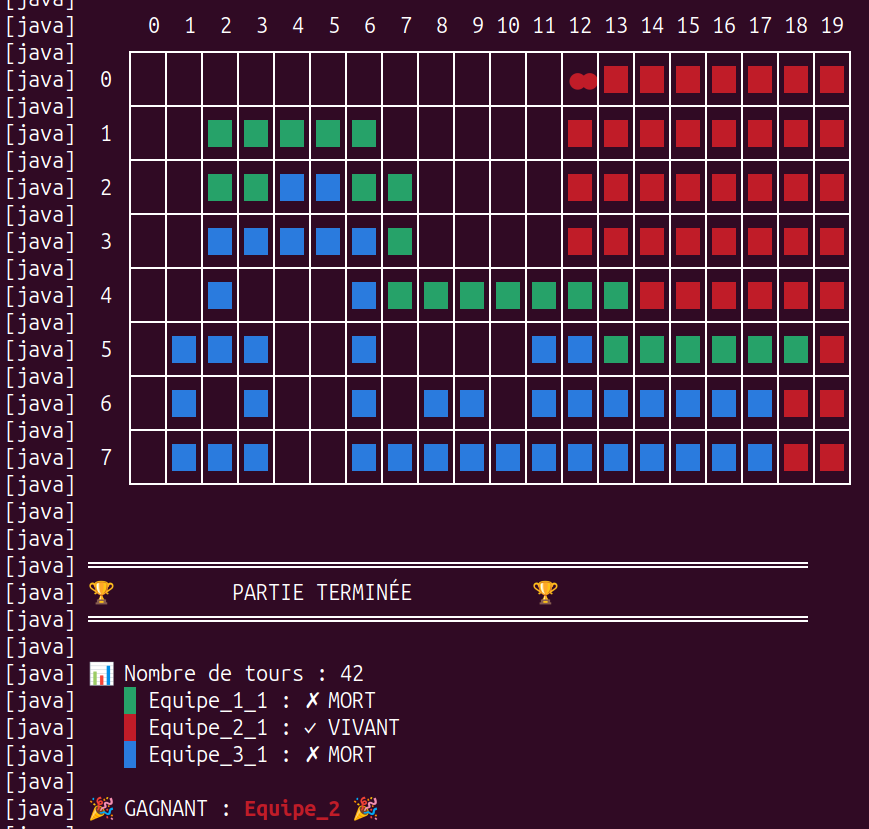
\includegraphics[width=0.9\linewidth, height=1\paperheight, keepaspectratio]{images/console.png}
    \caption{Une illustration d'une partie en mode console}
\end{figure}

\subsection{Interface graphique (GUI)}

Développée avec la bibliothèque \textbf{Swing}, l’interface graphique offre une immersion complète dans le jeu. Elle s’organise autour de plusieurs zones complémentaires. Au centre, le plateau de jeu est représenté sous la forme d’une grille dynamique qui affiche les joueurs, leurs positions respectives ainsi que les murs laissés au fil des déplacements. Cette représentation permet de suivre visuellement l’évolution de la partie et de mieux comprendre le comportement des différentes stratégies.

Autour de cette zone principale, l’interface intègre également un panneau de contrôle qui permet de démarrer, mettre en pause ou réinitialiser une partie. Ce panneau donne aussi accès à certains réglages, comme la vitesse de simulation, ce qui rend les tests plus souples et plus faciles à observer. Enfin, l’interface affiche des informations complémentaires en temps réel, notamment l’historique récent de la partie, certains résultats intermédiaires et différents éléments utiles au suivi des actions effectuées pendant le jeu.

\begin{figure}[H]
    \centering
    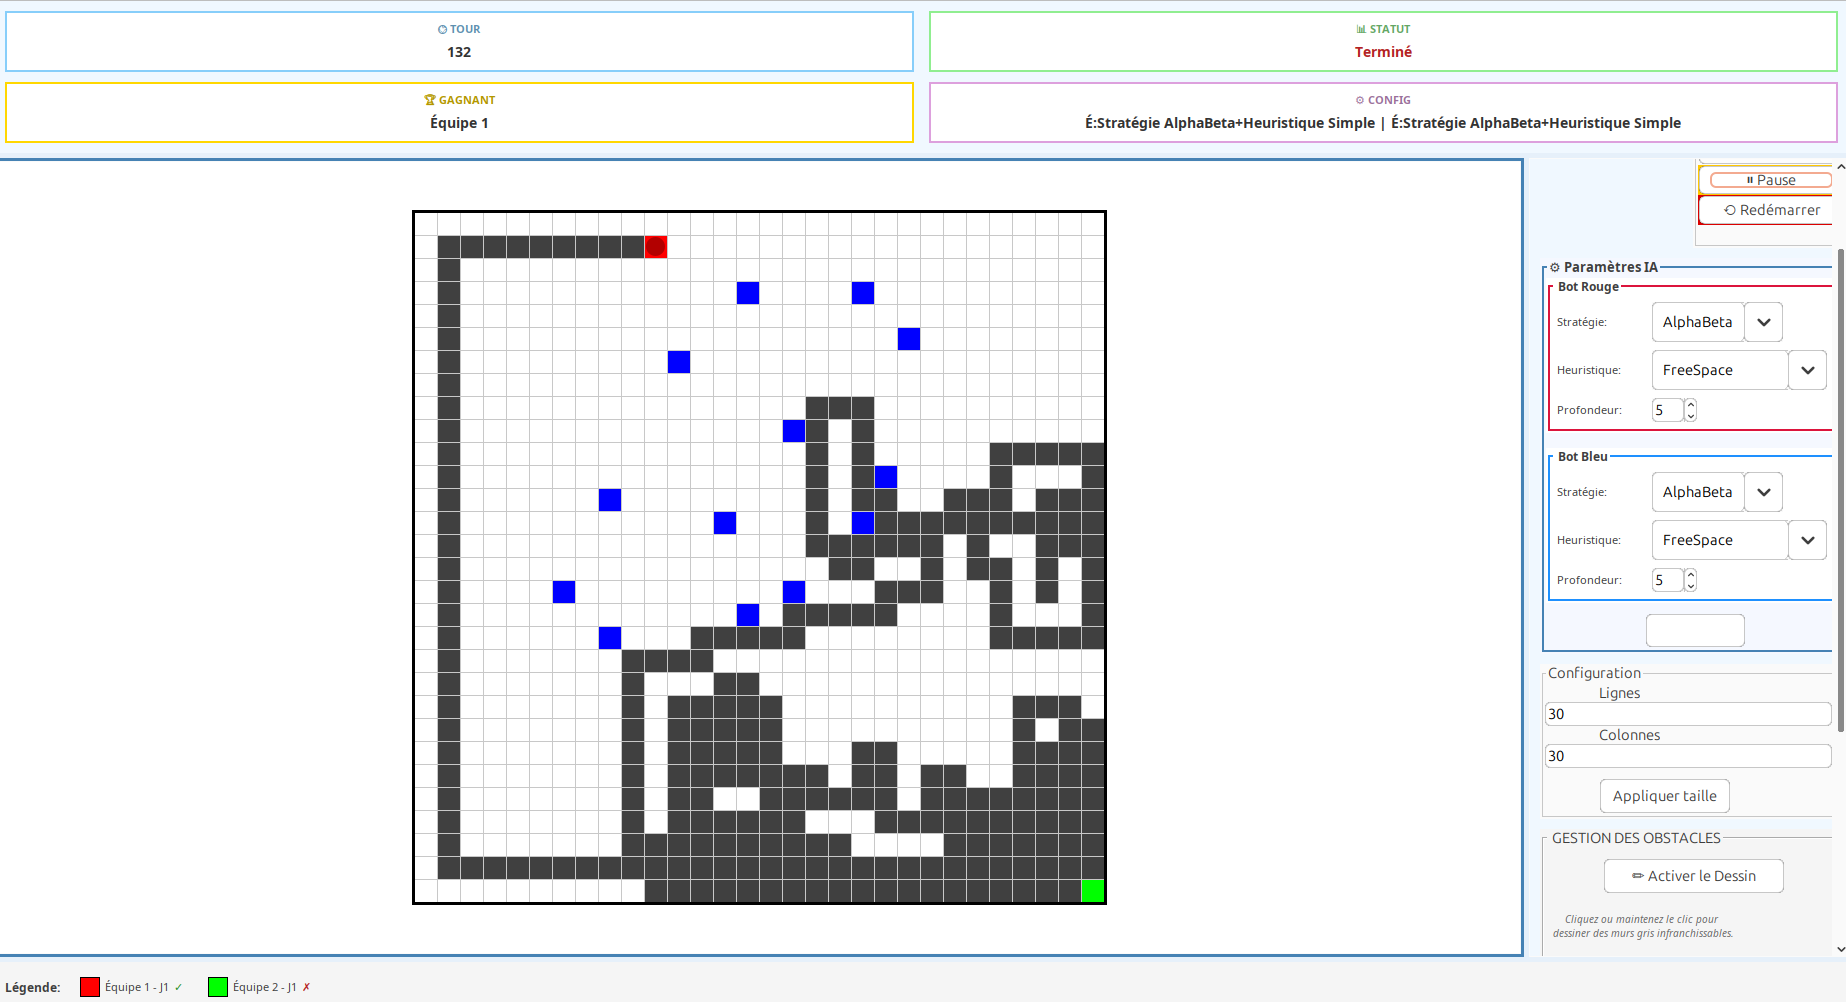
\includegraphics[width=1\linewidth, height=0.8\paperheight, keepaspectratio]{images/gui.png}
    \caption{Aperçu de l'interface graphique Swing}
\end{figure}

\subsection{Campagnes d'analyse et expérimentations}

Le volet expérimental constitue une partie importante du projet, car il permet d’évaluer les performances des différentes stratégies dans un cadre automatisé. Il repose principalement sur le package \texttt{experiment}, qui prend en charge l’organisation des campagnes de tests, l’exécution des parties et la récupération des résultats.

Le protocole expérimental consiste à lancer un grand nombre de parties entre différentes configurations d’algorithmes. Cela permet de comparer plusieurs stratégies, comme \texttt{MinMaxStrategie}, \texttt{MaxNStrategie}, \texttt{ParanoidStrategie} ou \texttt{SOSStrategie}, ainsi que plusieurs heuristiques d’évaluation. Chaque partie produit ensuite un objet \texttt{GameResult}, qui contient les informations essentielles pour l’analyse, comme l’équipe gagnante, le nombre de tours joués et le temps moyen de calcul.

Une fois les résultats récupérés, ils sont exportés dans des fichiers CSV, puis exploités pour construire des graphiques et des tableaux comparatifs. Cette étape rend possible une analyse plus globale des performances observées, notamment pour étudier l’effet de la profondeur de recherche, du choix de l’heuristique ou encore de la taille du plateau sur le comportement des intelligences artificielles.

\section{Analyse des expérimentations des Algorithmes}
\subsection{Présentation des expériences}

L’analyse présentée ici repose sur les résultats obtenus après les campagnes d’expérimentations automatiques lancées dans le projet. Les données ont ensuite été regroupées et visualisées sous forme de graphiques afin de mieux comparer les stratégies, les heuristiques, la profondeur de recherche et la taille du plateau.

Les graphiques permettent de voir rapidement les tendances générales. Ils ne servent pas seulement à compter le nombre de victoires, mais aussi à observer l’effet de certains paramètres sur le comportement global des stratégies. Dans cette partie, nous nous appuyons donc sur les résultats effectivement produits par le projet et sur les graphiques générés à partir des fichiers de sortie.
\begin{figure} [H]
    \centering
    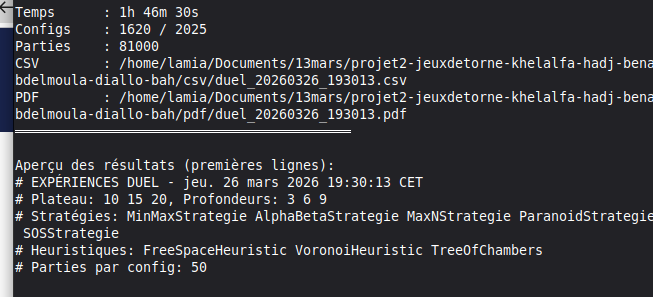
\includegraphics[width=1\linewidth, height=0.75\paperheight, keepaspectratio]{images/fin.png}
\end{figure}

\subsection{1ère partie d'analyse et d'expérimentation }

Cette section présente les résultats des simulations effectuées pour comparer les performances des différentes stratégies d'intelligence artificielle couplées à l'heuristique de \textbf{Voronoi (VoH)}. L'objectif est d'évaluer la robustesse des algorithmes à travers des indicateurs de performance et de fiabilité statistique.

\subsubsection{Méthodologie et Fiabilité Statistique}
Pour garantir la validité scientifique de nos tests, nous avons introduit un \textbf{intervalle de confiance} (marge d'erreur) pour chaque session de test. 

\begin{itemize}
    \item \textbf{Loi des grands nombres :} Plus le nombre de parties augmente, plus la marge d'erreur diminue. Par exemple, pour 200 parties, la confiance globale est de $\pm 6,06\%$, alors qu'elle monte à $\pm 30,59\%$ pour seulement 6 parties.
    \item \textbf{Stabilité :} La marge d'erreur globale sur l'ensemble des tests est de $\pm 5,33\%$, ce qui confère une grande fiabilité aux conclusions tirées sur l'équipe dominante.
\end{itemize}

\subsubsection{Résultats des Sessions (Confiance Détaillée)}

Le tableau suivant récapitule les taux de victoire de chaque configuration d'équipe (Algorithme $|$ Heuristique) avec leur marge d'erreur respective :

\begin{figure}[h]
    \centering
    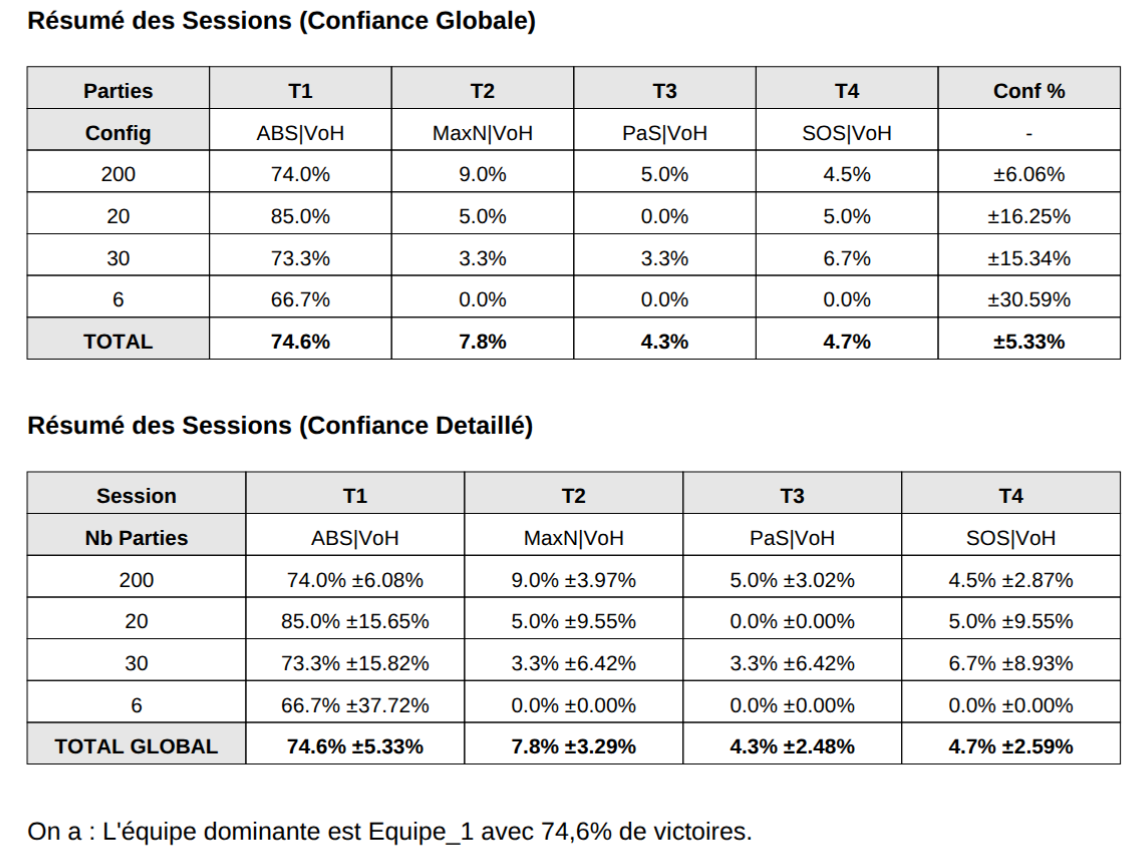
\includegraphics[width=0.9\linewidth]{images/analyse.png}
    \caption{Visualisation des sessions et de la confiance globale}
\end{figure}

\vspace{2cm}
\subsubsection{Interprétation et Conclusion}
L'analyse des données permet de tirer les conclusions suivantes :
\begin{enumerate}
    \item \textbf{Domination de l'Alpha-Beta (T1) :} Avec un taux de victoire final de $74,6\%$, l'algorithme Alpha-Beta surclasse nettement les autres stratégies lorsqu'il utilise l'heuristique de Voronoi.
    \item \textbf{Performance des stratégies N-joueurs :} Les algorithmes MaxN ($7,8\%$), SOS ($4,7\%$) et Paranoid ($4,3\%$) montrent des performances similaires et très en retrait par rapport à T1 dans ce contexte de duel ou de confrontation directe.
    \item \textbf{Validation :} L'équipe dominante est statistiquement identifiée comme étant l'Équipe 1 (ABS) avec une avance significative qui dépasse largement la marge d'erreur calculée.
\end{enumerate}

\subsection{2ème partie d'analyse et d'expérimentation (par stratégie)}
Dans l’ensemble, les résultats montrent que les performances ne dépendent pas d’un seul paramètre. Le choix de la stratégie a un effet important, mais il ne peut pas être séparé du choix de l’heuristique. On observe aussi que certaines profondeurs donnent de meilleurs résultats que d’autres, alors que la taille du plateau semble avoir un impact plus limité sur les tendances générales.

Les graphiques montrent surtout que les écarts les plus visibles viennent de la stratégie utilisée et de la qualité de l’heuristique. Certaines combinaisons donnent des résultats nettement meilleurs, alors que d’autres restent plus irrégulières ou produisent davantage de matchs nuls.

\vspace{1cm}
L’analyse par stratégie permet de comparer plus précisément le comportement de chaque algorithme. Le graphique suivant résume les résultats obtenus selon la stratégie utilisée.

\begin{figure}[H]
    \centering
    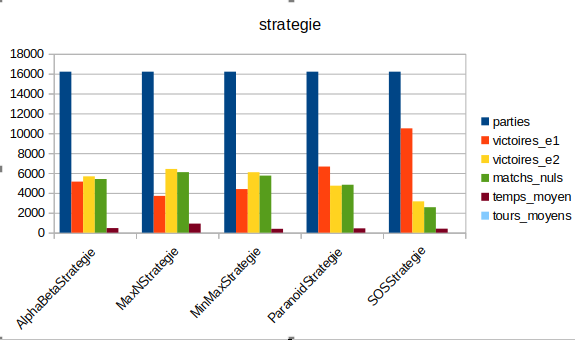
\includegraphics[width=0.92\textwidth]{images/strategie.png}
    \caption{Comparaison globale des stratégies}
    \label{fig:strategie}
\end{figure}

Sur la figure \ref{fig:strategie}, on remarque que les stratégies ne se comportent pas toutes de la même manière. Certaines gagnent plus souvent, d’autres produisent plus de matchs nuls, et certaines semblent plus dépendre du contexte. Le nombre de parties jouées est comparable entre les stratégies, ce qui permet de faire une comparaison assez équilibrée.

\subsubsection{MinMaxStrategie}

MinMaxStrategie donne des résultats globalement corrects, sans être la stratégie la plus dominante. Elle obtient un nombre de victoires raisonnable, mais reste derrière les meilleures configurations observées. Son comportement paraît assez stable, avec peu de résultats extrêmes. Cela confirme que MinMax reste une base classique et sérieuse, mais que son efficacité dépend beaucoup de l’évaluation utilisée.

\subsubsection{AlphaBetaStrategie}

AlphaBetaStrategie donne elle aussi des résultats solides. Son intérêt principal est de conserver une logique proche de MinMax tout en réduisant le coût de calcul grâce à l’élagage. Dans les résultats observés, elle reste compétitive et garde un bon niveau général. Elle apparaît comme une stratégie équilibrée, capable de produire de bons résultats sans être systématiquement la meilleure dans tous les cas.

\subsubsection{MaxNStrategie}

MaxNStrategie obtient des résultats plus mitigés. Le graphique montre qu’elle peut gagner dans certains cas, mais qu’elle reste globalement moins convaincante que les stratégies les plus performantes. Ce résultat n’est pas forcément surprenant, car MaxN est surtout pensé pour des contextes multi-joueurs. Dans un cadre plus restreint ou plus compétitif, son comportement semble moins directement efficace.

\subsubsection{ParanoidStrategie}

ParanoidStrategie ressort comme l’une des stratégies les plus fortes dans les résultats observés. Elle obtient un nombre de victoires élevé et semble mieux transformer les parties en résultats favorables. Son approche plus prudente et plus défensive paraît bien fonctionner dans le jeu de Tron, où la gestion de l’espace est essentielle. Cette stratégie semble donc particulièrement intéressante dans les configurations testées.

\subsection{Impact des heuristiques}

L’effet des heuristiques est très visible dans les résultats. Le graphique ci-dessous montre clairement que toutes les heuristiques n’apportent pas le même niveau de qualité aux stratégies.

\begin{figure}[H]
    \centering
    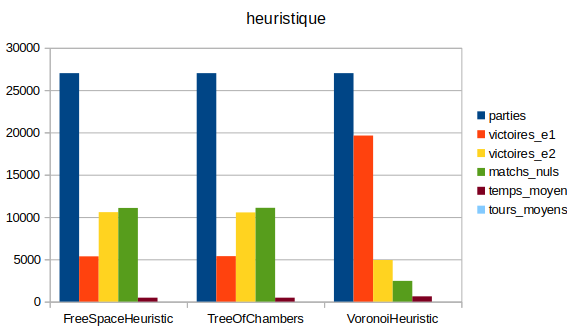
\includegraphics[width=0.78\textwidth]{images/heuristique.png}
    \caption{Comparaison des heuristiques selon les stratégies}
    \label{fig:heuristique}
\end{figure}

La figure \ref{fig:heuristique} met en évidence une tendance très nette : \textbf{VoronoiHeuristic} donne de meilleurs résultats que les autres heuristiques dans presque tous les cas. Elle se détache clairement pour chaque stratégie affichée. À l’inverse, \textbf{FreeSpaceHeuristic} et \textbf{TreeOfChambers} donnent des résultats plus faibles et souvent assez proches l’une de l’autre.

Cela montre que l’heuristique joue un rôle central. Même une bonne stratégie perd une grande partie de son intérêt si la fonction d’évaluation utilisée n’est pas assez pertinente. Dans ce projet, Voronoi semble être l’heuristique la plus adaptée pour représenter le contrôle de l’espace sur le plateau.

\subsection{Impact de la profondeur}

La profondeur de recherche a également une influence sur les résultats. Le graphique suivant permet de comparer les performances observées selon les différentes profondeurs testées.

\begin{figure}[H]
    \centering
    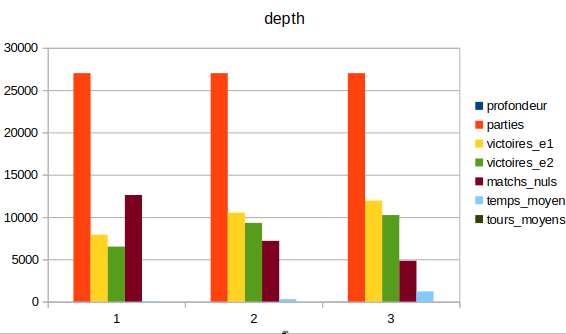
\includegraphics[width=0.92\textwidth]{images/depth.png}
    \caption{Impact de la profondeur de recherche}
    \label{fig:profondeur}
\end{figure}

La figure \ref{fig:profondeur} montre que la profondeur a bien un effet, mais que cet effet n’est pas totalement linéaire. La profondeur la plus élevée testée dans ce graphique semble produire davantage de victoires et moins de matchs nuls que les autres. En revanche, elle s’accompagne aussi d’un coût plus important en temps moyen et en nombre de tours moyens.

Cela veut dire qu’augmenter la profondeur peut améliorer la qualité de décision, mais que cela augmente aussi le coût de calcul. Le gain n’est donc pas gratuit. Dans le cadre du projet, on peut dire qu’une profondeur plus grande peut être utile, mais seulement si le temps d’exécution reste acceptable.

\subsection{Impact de la taille du plateau}

La taille du plateau modifie elle aussi le comportement global des parties, mais l’effet visible dans les résultats semble moins marqué que celui de la stratégie ou de l’heuristique.

\begin{figure}[H]
    \centering
    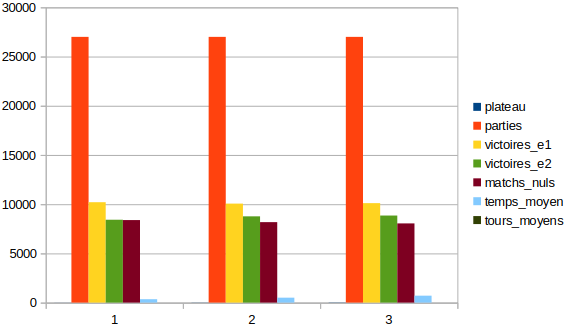
\includegraphics[width=0.92\textwidth]{images/plateau.png}
    \caption{Impact de la taille du plateau}
    \label{fig:plateau}
\end{figure}

Sur la figure \ref{fig:plateau}, les résultats restent assez proches d’un plateau à l’autre. Le nombre de parties, de victoires et de matchs nuls ne change pas fortement entre les trois cas affichés. En revanche, on remarque que le temps moyen et le nombre moyen de tours ont tendance à augmenter lorsque la taille du plateau augmente. Cela est logique, car un plateau plus grand laisse plus d’espace aux joueurs et peut prolonger les affrontements.

On peut donc dire que la taille du plateau joue surtout sur la durée et le rythme de la partie, mais qu’elle ne change pas complètement la hiérarchie générale observée entre les stratégies et les heuristiques.

\subsection{Synthèse et réponse à la question scientifique}

Les résultats permettent de dégager plusieurs conclusions simples. D’abord, le facteur le plus visible dans cette campagne d’expérimentation est l’heuristique. Le graphique des heuristiques montre clairement que \textbf{VoronoiHeuristic} domine les autres. Ensuite, du côté des stratégies, \textbf{ParanoidStrategie} ressort comme l’une des plus efficaces dans les configurations observées.

L’analyse de la profondeur montre aussi qu’une recherche plus poussée peut améliorer les résultats, mais au prix d’un temps de calcul plus élevé. Enfin, la taille du plateau semble avoir un effet plus limité sur les performances globales, même si elle influence la durée des parties.

La réponse à la question scientifique peut donc être formulée ainsi : dans ce projet, la profondeur de recherche a bien une influence, mais son effet reste moins important que celui de la stratégie et surtout de l’heuristique. Une profondeur plus grande peut aider, mais elle n’est réellement intéressante que si elle s’appuie sur une bonne évaluation du plateau.
\subsection{Limites et perspectives}

Les résultats présentés dans cette partie doivent avant tout être compris comme des résultats \textbf{indicatifs}. Ils permettent de dégager des tendances générales et de comparer plusieurs comportements, mais ils ne suffisent pas encore à établir des conclusions définitives sur toutes les dimensions du projet. En effet, les expériences réalisées ici ne couvrent qu’une partie des possibilités offertes par le jeu et par les stratégies implémentées.

Pour aller plus loin, il serait nécessaire d’enrichir le protocole expérimental. Par exemple, il serait intéressant de tester plus précisément l’impact de la \textbf{taille des équipes} et du \textbf{nombre total de joueurs} sur les performances observées. Cela permettrait de mieux comprendre comment les stratégies évoluent lorsque la dynamique de jeu devient réellement multi-joueurs. Il serait également pertinent d’étudier plus directement les \textbf{alliances} et les comportements de coalition, en particulier pour les stratégies comme SOS, qui prennent tout leur sens dans ce type de contexte.

D’autres améliorations seraient aussi possibles, comme l’ajout de nouvelles profondeurs de recherche, l’étude de davantage de tailles de plateau, ou encore la mise en place d’outils d’analyse plus précis pour comparer les résultats. Ainsi, cette première campagne d’expérimentations constitue surtout une base de travail solide, mais elle demande encore à être approfondie pour exploiter pleinement tout le potentiel du projet.

\section{Tests}
\subsection{Stratégie de test}

La stratégie de test adoptée dans le projet repose principalement sur des tests unitaires ciblant le modèle, les heuristiques et plusieurs stratégies d'intelligence artificielle. L'objectif était de vérifier le comportement général des composants avant de les intégrer dans des parties complètes. Ce choix est cohérent avec la structure du projet, car la majorité de la logique critique se trouve dans le package \texttt{model}.

Les tests ne remplacent évidemment pas l'observation d'une partie réelle ni l'analyse expérimentale, mais ils constituent une première garantie de bon fonctionnement pour les briques de base.

\subsection{Tests unitaires}

Le package \texttt{test} contient en particulier des classes comme \texttt{ModeleJeuTest}, \texttt{MinMaxStrategieTest}, \\\texttt{AlphaBetaStrategieTest}, \texttt{ParanoidStrategieTest}, \texttt{SOSStrategieTest}, \texttt{FreeSpaceHeuristicTest}, \\\texttt{VoronoiHeuristicTest} et \texttt{TreeOfChambersHeuristicTest}. L'ensemble est exécuté via JUnit 4, présent dans le répertoire \texttt{lib}. Cette couverture montre que le projet ne s'est pas limité à une validation visuelle du jeu, mais a intégré un minimum d'automatisation dans la vérification du code.

Les tests portent en particulier sur la validité des directions proposées, la cohérence de certaines évaluations heuristiques et le comportement global du modèle dans des situations simples. Ils offrent une base utile, même si certaines propriétés plus complexes du jeu restent difficiles à vérifier uniquement par des tests unitaires.

\subsection{Validation}

La validation du projet s'est faite à deux niveaux. D'une part, les tests unitaires ont permis de contrôler plusieurs composants isolés. D'autre part, l'exécution de parties via l'interface et via le module d'expérimentation a rendu possible une validation empirique de l'ensemble. Cette double approche est importante dans un projet de simulation, car un algorithme peut être correct au niveau syntaxique tout en produisant un comportement peu crédible si l'intégration générale du système est défaillante.

\section{Conclusion}

\subsection{Bilan et Objectifs atteints}
Le projet a abouti à une plateforme de simulation complète, alliant rigueur logicielle et capacités expérimentales. Les objectifs initiaux ont été pleinement remplis :
\begin{itemize}
    \item \textbf{Architecture robuste :} Une séparation stricte (MVC/Observer) permettant d'isoler la logique métier du rendu graphique.
    \item \textbf{Intelligence Artificielle :} Implémentation fonctionnelle de plusieurs algorithmes de recherche (\textit{Minimax, Alpha-Beta, MaxN, Paranoid, SOS}) et d'heuristiques spatiales (\textit{Voronoi, Tree of Chambers}).
    \item \textbf{Pipeline de données :} Capacité à générer des campagnes d'expérimentation massives, de l'exécution brute à l'analyse graphique automatisée.
\end{itemize}

\subsection{Difficultés et Enseignements}
Le développement a révélé des défis techniques et conceptuels majeurs :
\begin{itemize}
    \item \textbf{Complexité algorithmique :} Maintenir une architecture propre tout en intégrant des logiques de recherche variées a nécessité une abstraction poussée des stratégies.
    \item \textbf{Rigueur expérimentale :} L'aspect aléatoire des positions de départ a imposé la mise en place d'un protocole de duel strict (50 parties par configuration) pour obtenir des statistiques significatives.
    \item \textbf{Optimisation :} La gestion du multithreading pour les simulations intensives a représenté un défi technique pour garantir l'isolation des données et la cohérence des résultats.
\end{itemize}

\subsection{Perspectives}
Le moteur de jeu constitue une base solide pour des évolutions futures :
\begin{itemize}
    \item \textbf{Extension multi-agent :} Approfondir les tests en configuration "équipes contre équipes" pour évaluer la coopération entre IA.
    \item \textbf{Affinement du protocole :} Réduire l'influence de l'aléatoire en utilisant des scénarios de départ prédéfinis.
    \item \textbf{Heuristiques avancées :} Intégrer de nouveaux modèles d'évaluation basés sur l'apprentissage ou une analyse topologique encore plus fine du plateau.
\end{itemize}

\vspace{1cm}
\begin{center}
    \textit{Ce projet démontre qu'au-delà du jeu, le Tron est un excellent support pour l'étude des systèmes multi-agents et des stratégies de contrôle spatial en temps limité.}
\end{center}



\clearpage

\begin{thebibliography}{9}

\bibitem{minmax}
Russell, S., Norvig, P. (2010). \textit{Artificial Intelligence: A Modern Approach}. Prentice Hall.

\bibitem{sos}
Sturtevant, N. (2003). \textit{Last-Branch and Speculative Pruning Algorithms for Maxn}. AAAI.

\bibitem{kang}
Kang, L. (2022). \textit{Heuristic Tree of Chambers for the Game of Tron}. Maastricht University. \url{https://project.dke.maastrichtuniversity.nl/games/files/bsc/Kang_Bsc-paper.pdf}

\bibitem{tron}
Tron Game. \textit{Wikipedia}. \url{https://en.wikipedia.org/wiki/Tron_(video_game)}

\bibitem{voronoi}
Voronoi Diagram. \textit{Wikipedia}. \url{https://en.wikipedia.org/wiki/Voronoi_diagram}

\end{thebibliography}

\end{document}